\chapter{Approximation, Asymptotics and Root Finding}\label{ch:asymptotics}

\begin{chapterintro}
Almost nothing in the paper can be computed with pencil and paper alone. The smooth zeros $s_n$ are defined as the solutions of an equation, $\Nsm(s_n)=n-\tfrac12$, that has no solution in terms of logarithms and powers. The Wu--Sprung potential is defined backwards: the paper gives the position $x$ as a function of the height $V$, and the computer has to turn this around to get $V$ as a function of $x$. The truncated explicit formula predicts a zero by solving yet another equation. Every one of these steps is \emph{root finding}, and the paper names the algorithm it uses: Brent's method.

Before you can find a root you need to know roughly where it is, and before you can trust a number you need to know how large its error is. So this chapter has three threads. The first is \emph{asymptotics}: the language of big-O, little-o and $\sim$, which lets you say precisely that one quantity grows like another, and the tools (sums compared with integrals, Stirling's formula for factorials and the Gamma function) that produce such statements. The second is \emph{root finding}: inverting monotone functions, bisection with a guaranteed error bound, Newton's method with its very fast convergence, and Brent's method, which combines the safety of the first with the speed of the second. The third is \emph{trust}: absolute and relative errors, significant digits, and the floating-point numbers that computers actually use, including the surprising fact that a quantity that is exactly zero on paper can come out of a computer as a number of size $10^{-7}$.

Where this shows up in the paper: solving Eq.~(1) for the smooth zeros (Sec.~II~A and Appendix~A step 2), inverting Eq.~(2) (Sec.~II~B, Appendix~A step 3), solving the oracle's level equation with Brent's method bracketed by $\pm3$ around the smooth zero (Appendix~A step 8), the Lambert-$W$ form of the smooth zeros mentioned in Sec.~I~A, the root ambiguity flagged in Table~IV, and the float32 noise artifact that manufactured a spurious result in Sec.~V.
\end{chapterintro}

\begin{prerequisites}
\item Chapter~\ref{ch:complex}: the Taylor series of $e^x$; complex numbers, modulus and argument, the logarithm of a complex number and its branches (the last three are needed only for one box on the complex Gamma function).
\item Chapter~\ref{ch:series}: limits of sequences, partial sums, the geometric series, the Taylor series of $\log(1-x)$, the integral test.
\item First-year calculus: derivatives (chain and product rules), integrals, integration by parts, substitution, the tangent line to a graph, the Taylor series of $\sin x$ and $\cos x$.
\item Throughout, $\log$ means the natural logarithm, as in the paper.
\end{prerequisites}

%======================================================================
\section{Errors, relative errors and significant digits}\label{sec:asymptotics-errors}

Every number a computer gives you is an approximation. Even the first Riemann zero, which the paper quotes as $t_1=14.134725141734695$ (Sec.~II~A), is a rounded version of an infinitely long decimal. Before we can talk about how good an approximation is, we need words for the size of the mistake.

\subsection{Absolute and relative error}

Let $x$ be a true value and $\hat x$ an approximation to it.

\paragraph{Definition.} The \emph{absolute error} is $\hat x - x$ (sometimes its magnitude $\abs{\hat x-x}$ is meant). The \emph{relative error} is
\begin{equation}
\epsilon_{\rm rel}=\frac{\hat x - x}{x}\qquad (x\neq 0).
\label{eq:asymptotics-relerr}
\end{equation}

The absolute error carries the units of $x$; the relative error is a pure number. Which one matters depends on the question. If you measure the length of a football field to within $1\,$cm you have done very well; if you measure the thickness of a coin to within $1\,$cm you have learned nothing. The absolute errors are the same; the relative errors differ by a factor of about $50\,000$ (about $10^{-4}$ for a $100\,$m field against about $5$ for a $2\,$mm coin).

\paragraph{Errors in natural units.} Physicists often measure an error in units of some natural scale of the problem. For the zeta zeros the natural scale is the \emph{local mean spacing}: the typical distance between neighboring zeros near a given height. The paper writes it $\gap_n$ and quotes every error in these units (``all errors below are quoted in units of the local mean spacing'', Sec.~II~A). We derive the formula $\gap_n=2\pi/\log(s_n/2\pi)$ in \cref{sec:asymptotics-inverse}; for now, all you need is that near the first zero the mean spacing is about $7.500$, and near the thousandth zero it is about $1.159$. An error of $0.01$ in $t$ is therefore a much larger fraction of a spacing at the thousandth zero than at the first.

\subsection{Significant digits}

\paragraph{Definition.} A number written in decimal has $d$ \emph{significant digits} if it is written with $d$ digits starting from the first nonzero one. When a true value $x$ is rounded to $d$ significant digits, the rounding changes it by at most half a unit in the last place kept, and the relative error then satisfies (proof immediately below)
\begin{equation}
\abs{\epsilon_{\rm rel}}\le 5\times10^{-d}.
\label{eq:asymptotics-sigdig}
\end{equation}
Here is why. Write $x=m\times10^{q}$ with $1\le m<10$ and $q$ an integer. Keeping $d$ significant digits means keeping $m$ to $d-1$ decimal places, so the rounding error in $m$ is at most $\tfrac12\times10^{-(d-1)}=5\times10^{-d}$. The absolute error in $x$ is therefore at most $5\times10^{-d}\times10^{q}$, and dividing by $\abs{x}=m\times10^q\ge 10^q$ gives \cref{eq:asymptotics-sigdig}.

Conversely, we say loosely that an approximation is ``good to $d$ significant digits'' when its relative error is about $10^{-d}$ or smaller.

\begin{sample}{How wrong is $t_1\approx 14.13$?}
The first zero is $t_1=14.134725141734695$ (paper, Sec.~II~A). You round it to $14.13$. Find the absolute error, the relative error, and the error in units of the local mean spacing $\gap_1=7.500$ (derived in \cref{sec:asymptotics-inverse}).

\textbf{Step 1:} Absolute error: $14.13-14.134725=-0.004725$, so $\abs{\hat x-x}=0.004725$.

\textbf{Step 2:} Relative error: $0.004725/14.134725=3.34\times10^{-4}$. This is below the bound $5\times10^{-4}$ of \cref{eq:asymptotics-sigdig} for $d=4$ digits, as it must be.

\textbf{Step 3:} In mean spacings: $0.004725/7.500=6.30\times10^{-4}$.

\[
\boxed{\abs{\Delta t}=0.004725,\quad \abs{\epsilon_{\rm rel}}=3.34\times10^{-4},\quad 6.30\times10^{-4}\text{ spacings}}
\]
Even a crude four-digit value of $t_1$ is accurate to better than a thousandth of a spacing. The paper's quoted rms errors (such as $0.263$ spacings) are hundreds of times larger, so they are not rounding effects.
\end{sample}

\begin{checkpoint}
A friend reports an error of $0.001$ in a computed zero and says ``that is negligible''. What extra information do you need before agreeing?
\end{checkpoint}
\checkanswer{You need a scale. An absolute error of $0.001$ is negligible compared with the mean spacing ($7.5$ near $t_1$, about $1.16$ near $t_{1000}$) but would be enormous if the quantity were itself of size $10^{-4}$. Ask for the relative error or the error in mean spacings.}

\begin{keyideas}
\item Absolute error $\hat x-x$ has units; relative error $(\hat x-x)/x$ is dimensionless, \cref{eq:asymptotics-relerr}.
\item Rounding to $d$ significant digits gives a relative error at most $5\times10^{-d}$, \cref{eq:asymptotics-sigdig}.
\item The paper measures errors in units of the local mean spacing $\gap_n$, a natural scale that shrinks with height.
\end{keyideas}

%======================================================================
\section{Orders of growth: $\order$, $o$ and $\sim$}\label{sec:asymptotics-order}
% DYK-BEGIN
\begin{didyouknow}{Big O Is Older Than Computers}
The symbol $\mathcal{O}$ was introduced by Paul Bachmann in an 1894 book on analytic number theory. Edmund Landau made it famous in his 1909 treatise on the distribution of primes, which is why $\mathcal{O}$ and $o$ are called Landau symbols. Only in 1976 did Donald Knuth standardize $\Omega$ and $\Theta$ for computer science. Asymptotic notation was born in the study of primes.
\end{didyouknow}
% DYK-END

The smooth counting function of the paper, Eq.~(1),
\begin{equation}
\Nsm(t)=\frac{t}{2\pi}\log\frac{t}{2\pi}-\frac{t}{2\pi}+\frac78,
\label{eq:asymptotics-nsm}
\end{equation}
has three terms. Which one matters most for large $t$? How fast does the whole thing grow? To answer such questions crisply, mathematicians and physicists use three symbols.

\subsection{Definitions}

Let $f(t)$ and $g(t)$ be functions defined for large $t$, with $g(t)\neq0$ there.

\paragraph{Big-O.} We write $f(t)=\order(g(t))$ as $t\to\infty$ if there are constants $C>0$ and $t_0$ such that
\begin{equation}
\abs{f(t)}\le C\,\abs{g(t)}\qquad\text{for all } t\ge t_0.
\label{eq:asymptotics-bigO}
\end{equation}
In words: $f$ grows no faster than a fixed multiple of $g$.

\paragraph{Little-o.} We write $f(t)=o(g(t))$ as $t\to\infty$ if
\begin{equation}
\lim_{t\to\infty}\frac{f(t)}{g(t)}=0.
\label{eq:asymptotics-littleo}
\end{equation}
In words: $f$ becomes negligible compared with $g$.

\paragraph{Asymptotic equivalence.} We write $f(t)\sim g(t)$ as $t\to\infty$ if
\begin{equation}
\lim_{t\to\infty}\frac{f(t)}{g(t)}=1.
\label{eq:asymptotics-sim}
\end{equation}
Equivalently, $f(t)=g(t)+o(g(t))$: the relative difference goes to zero.

The same symbols are used as $x\to0$ with ``for all $t\ge t_0$'' replaced by ``for all $0<\abs{x}\le x_0$''. For example, from the Taylor series $\cos x=1-x^2/2+x^4/24-\cdots$ we have $1-\cos x=\tfrac12x^2+\order(x^4)$ as $x\to0$.

\subsection{Examples and rules}

\begin{itemize}
\item $5t^2+3t=\order(t^2)$: for $t\ge1$, $3t\le3t^2$, so $\abs{5t^2+3t}\le 8t^2$; take $C=8$, $t_0=1$.
\item $5t^2+3t\sim 5t^2$, since $(5t^2+3t)/(5t^2)=1+3/(5t)\to1$.
\item $\sin t=\order(1)$, because $\abs{\sin t}\le1$.
\item $t^2+t\sim t^2$ but the difference $(t^2+t)-t^2=t$ grows without bound. \emph{Asymptotic equivalence controls the ratio, not the difference.}
\end{itemize}

Three rules follow directly from the definitions. If $f_1=\order(g)$ and $f_2=\order(g)$ then $f_1+f_2=\order(g)$ (add the two inequalities and use the larger $t_0$; the constant becomes $C_1+C_2$). If $f_1=\order(g_1)$ and $f_2=\order(g_2)$ then $f_1f_2=\order(g_1g_2)$ (multiply the inequalities; the constant becomes $C_1C_2$). And $o(g)$ implies $\order(g)$ (if the ratio tends to zero it is eventually below $1$).

\begin{pitfall}
The equals sign in $f=\order(g)$ is a one-way statement. We write $t=\order(t^2)$ and $t^2=\order(t^2)$, but you may not conclude $t=t^2$. Read ``$=\order(g)$'' as ``is a function bounded by a multiple of $g$''.
\end{pitfall}

\subsection{Logarithms lose to every power}

The single most useful fact about growth rates in this book is:
\begin{equation}
\log t=o(t^{a})\quad\text{as } t\to\infty,\ \text{for every } a>0.
\label{eq:asymptotics-logpower}
\end{equation}
\emph{Proof.} Substitute $t=e^u$, so $u=\log t\to\infty$ as $t\to\infty$ and $t^a=e^{au}$. We need $u/e^{au}\to0$. The Taylor series $e^{y}=1+y+y^2/2+\cdots$ (Chapter~\ref{ch:complex}) has only positive terms when $y>0$, so $e^{y}>y^2/2$. With $y=au$:
\[
\frac{u}{e^{au}}<\frac{u}{(au)^2/2}=\frac{2}{a^2u}\longrightarrow 0.
\]
\hfill$\square$

Two relatives follow in the same way. First, for $y>0$ every term of the Taylor series of $e^y$ is positive, so $e^y>y^{k+1}/(k+1)!$ for any whole number $k\ge0$; hence $y^k/e^y<(k+1)!/y\to0$ as $y\to\infty$. This says that an exponential beats any power, $t^k=o(e^{t})$. Second, with $t=e^u$ and $y=au$, $(\log t)^k/t^a=u^k/e^{au}=a^{-k}\,y^k/e^y\to0$, so a power beats any power of a logarithm, $(\log t)^k=o(t^a)$.

\begin{pitfall}
``Eventually'' can be a long time. The ratio $\log t/t^{0.1}$ tends to zero, yet it first \emph{increases}: with $u=\log t$ the ratio is $u e^{-0.1u}$, whose derivative $e^{-0.1u}(1-0.1u)$ vanishes at $u=10$. The maximum, at $t=e^{10}\approx2.20\times10^{4}$, is $10/e=3.68$. Even at $t=10^{30}$ the ratio is still $0.069$. Asymptotic statements say nothing about the size of the constants or the place where the limit ``kicks in''.
\end{pitfall}

\subsection{Leading-order behavior}

The \emph{leading-order behavior} of $f$ is the simplest function $g$ with $f\sim g$. To find it, identify the term that dominates all others and check that the others are little-o of it.

\begin{sample}{Leading order of the smooth counting function}
Find the leading-order behavior of $\Nsm(t)$ in \cref{eq:asymptotics-nsm}, write the remainder with $\order$, and test how good the leading term is at the thousandth zero, $t_{1000}=1419.42248094599$ (paper, Sec.~II~A).

\textbf{Step 1:} Expand the logarithm: $\log(t/2\pi)=\log t-\log2\pi$. Then
\[
\Nsm(t)=\frac{t}{2\pi}\log t-\frac{t}{2\pi}\bigl(\log 2\pi+1\bigr)+\frac78 .
\]

\textbf{Step 2:} Compare each term with $\frac{t}{2\pi}\log t$. The second term divided by the first is $-(\log2\pi+1)/\log t\to0$. The third divided by the first is $\tfrac78\cdot2\pi/(t\log t)\to0$. So both are little-o of the first, and
\[
\Nsm(t)\sim\frac{t}{2\pi}\log t,\qquad \Nsm(t)=\frac{t}{2\pi}\log t+\order(t).
\]
(The remainder $-\frac{t}{2\pi}(\log2\pi+1)+\frac78$ is bounded by a constant times $t$ for $t\ge1$.)

\textbf{Step 3:} Evaluate at $t_{1000}$. Then $t/2\pi=225.908$, $\log(t/2\pi)=5.4201$, and \cref{eq:asymptotics-nsm} gives $\Nsm(t_{1000})=999.42$. The leading term gives $225.908\times\log(1419.42)=225.908\times7.2580=1639.6$.

\textbf{Step 4:} The ratio is $1639.6/999.42$:
\[
\boxed{\frac{(t/2\pi)\log t}{\Nsm(t)}\Big|_{t=t_{1000}}=1.64}
\]
So at the heights used in the paper, the ``leading term'' overestimates by 64\%. The ratio does tend to 1, but only as fast as $1/\log t$ shrinks, which is very slowly. This is why the paper always works with the full \cref{eq:asymptotics-nsm}, never with its leading term.
\end{sample}

\begin{checkpoint}
True or false: if $f\sim g$ then $f-g\to0$.
\end{checkpoint}
\checkanswer{False. $t^2+t\sim t^2$, but the difference is $t$, which grows. Only the ratio tends to 1.}

\subsection{Asymptotic expansions}

Often we can do better than the leading term. A sequence of ``gauge functions'' $\varphi_0(t),\varphi_1(t),\dots$ with $\varphi_{k+1}=o(\varphi_k)$ (for example $1,1/t,1/t^2,\dots$) defines an \emph{asymptotic expansion}
\[
f(t)\approx\sum_{k}a_k\varphi_k(t)
\]
when, for every $K$, the error after $K$ terms is $\order(\varphi_K)$:
$f(t)-\sum_{k=0}^{K-1}a_k\varphi_k(t)=\order(\varphi_K(t))$. The key point is that this is a statement about each \emph{fixed} truncation as $t\to\infty$, not about the infinite sum. Stirling's series in \cref{sec:asymptotics-stirling} is the classic example.

\begin{keyideas}
\item $f=\order(g)$: bounded by a multiple of $g$; $f=o(g)$: negligible relative to $g$; $f\sim g$: ratio tends to 1 (\cref{eq:asymptotics-bigO,eq:asymptotics-littleo,eq:asymptotics-sim}).
\item Logarithms grow more slowly than any positive power, \cref{eq:asymptotics-logpower}, but the crossover can be very late.
\item $\Nsm(t)\sim\frac{t}{2\pi}\log t$, yet at $t_{1000}$ the leading term is off by 64\%: logarithmic corrections converge slowly.
\end{keyideas}

%======================================================================
\section{Comparing sums with integrals}\label{sec:asymptotics-sums}

Sums are hard; integrals are easy. A sum of values of a smooth monotone function is squeezed between two integrals, and this squeeze is the source of many asymptotic formulas, including Stirling's.

\subsection{The squeeze}

\paragraph{Theorem (comparison of sums and integrals).} Let $f$ be positive and decreasing on $[1,\infty)$. Then for every integer $n\ge1$,
\begin{equation}
\int_1^{n+1}f(x)\,\dd x\;\le\;\sum_{k=1}^{n}f(k)\;\le\;f(1)+\int_1^{n}f(x)\,\dd x .
\label{eq:asymptotics-squeeze}
\end{equation}

\emph{Proof.} On the interval $[k,k+1]$ a decreasing function satisfies $f(k+1)\le f(x)\le f(k)$. Integrating over this unit-length interval,
\[
f(k+1)\le\int_k^{k+1}f(x)\,\dd x\le f(k).
\]
Sum the right inequality over $k=1,\dots,n$: $\int_1^{n+1}f\,\dd x\le\sum_{k=1}^n f(k)$, the left half of \cref{eq:asymptotics-squeeze}. Sum the left inequality over $k=1,\dots,n-1$: $\sum_{k=2}^{n}f(k)\le\int_1^{n}f\,\dd x$; add $f(1)$ to both sides to get the right half. \hfill$\square$

Geometrically (\cref{fig:asymptotics-sumint}), the sum is the total area of unit-width rectangles of heights $f(1),f(2),\dots$, which sit partly above and partly below the curve.

\begin{figure}[htbp]\centering
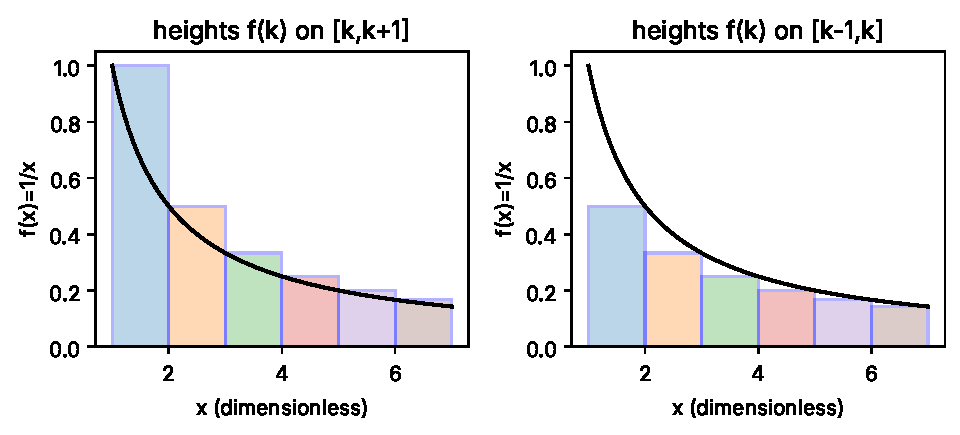
\includegraphics[width=0.85\linewidth]{figs/asymptotics_sumint.pdf}
\caption{Comparing a sum with an integral for the decreasing function $f(x)=1/x$. Left: rectangles of height $f(k)$ on $[k,k+1]$ lie above the curve, so $\sum_{k=1}^{n}f(k)\ge\int_1^{n+1}f\,\dd x$. Right: rectangles of height $f(k)$ on $[k-1,k]$ lie below the curve, so $\sum_{k=2}^{n}f(k)\le\int_1^{n}f\,\dd x$. The axes are dimensionless.}
\label{fig:asymptotics-sumint}
\end{figure}

For an \emph{increasing} positive function the inequalities reverse. On $[k,k+1]$ we now have $f(k)\le f(x)\le f(k+1)$, and the same summing gives
\begin{equation}
\int_1^{n}f(x)\,\dd x\;\le\;\sum_{k=2}^{n}f(k)\;\le\;\int_1^{n}f(x)\,\dd x+f(n)-f(1)\quad(f\text{ increasing}).
\label{eq:asymptotics-squeeze-inc}
\end{equation}
In detail: integrating $f(k)\le f(x)\le f(k+1)$ over the unit interval $[k,k+1]$ gives $f(k)\le\int_k^{k+1}f\,\dd x\le f(k+1)$. Summing the right inequality over $k=1,\dots,n-1$ gives $\int_1^nf\,\dd x\le\sum_{k=2}^{n}f(k)$, the left half of \cref{eq:asymptotics-squeeze-inc}. Summing the left inequality over $k=1,\dots,n-1$ gives $\sum_{k=1}^{n-1}f(k)\le\int_1^nf\,\dd x$; adding $f(n)-f(1)$ to both sides and using $\sum_{k=1}^{n-1}f(k)+f(n)-f(1)=\sum_{k=2}^{n}f(k)$ gives the right half.

\subsection{The harmonic numbers and Euler's constant}

The \emph{harmonic number} is $H_n=\sum_{k=1}^n1/k$. In Chapter~\ref{ch:series} you saw that $H_n\to\infty$. How fast? Apply \cref{eq:asymptotics-squeeze} with $f(x)=1/x$, using $\int_1^{X}\dd x/x=\log X$:
\begin{equation}
\log(n+1)\le H_n\le 1+\log n .
\label{eq:asymptotics-harmonic}
\end{equation}
Dividing by $\log n$ and letting $n\to\infty$ (note $\log(n+1)/\log n\to1$) squeezes $H_n/\log n\to1$: $H_n\sim\log n$.

The difference $\gamma_n=H_n-\log n$ actually converges (Problem~26 asks you to prove it). Its limit is \emph{Euler's constant} $\gamma=0.5772156649\ldots$ (a standard constant). \begin{beyond}
\textbf{Refining $H_n$.} Euler's summation formula expresses a sum $\sum_{k=1}^nf(k)$ as the integral $\int_1^nf\,\dd x$ plus correction terms built from $f$ and its derivatives at the endpoints. Applied to $f(x)=1/x$ it gives the expansion \cref{eq:asymptotics-Hn-expansion} below. We take it on trust; the proof is in \cite{apostol}.
\end{beyond}
\noindent The expansion, taken on trust as stated in the box, reads
\begin{equation}
H_n=\log n+\gamma+\frac{1}{2n}-\frac{1}{12n^2}+\order(n^{-4}).
\label{eq:asymptotics-Hn-expansion}
\end{equation}

\begin{sample}{Squeezing $H_{10}$}
Compute $H_{10}$ exactly, the bounds of \cref{eq:asymptotics-harmonic}, and the approximation \cref{eq:asymptotics-Hn-expansion}.

\textbf{Step 1:} $H_{10}=1+\tfrac12+\tfrac13+\dots+\tfrac1{10}=2.928968$.

\textbf{Step 2:} Bounds: $\log 11=2.397895$ and $1+\log10=3.302585$. Indeed $2.397895\le2.928968\le3.302585$.

\textbf{Step 3:} $H_{10}-\log10=2.928968-2.302585=0.626383$, still noticeably above $\gamma=0.577216$.

\textbf{Step 4:} With the correction terms: $2.302585+0.577216+0.05-0.000833=2.928968$, matching $H_{10}$ to all six decimals.

\[
\boxed{2.397895\le H_{10}=2.928968\le 3.302585}
\]
The crude squeeze pins $H_{10}$ to within about $\pm0.45$; the asymptotic expansion, even at $n=10$, is accurate to about $10^{-6}$.
\end{sample}

\subsection{The sum of logarithms}

The logarithm of a factorial is a sum: $\log n!=\log1+\log2+\dots+\log n=\sum_{k=2}^n\log k$ (the $k=1$ term is zero). Since $\log x$ is increasing, \cref{eq:asymptotics-squeeze-inc} applies. By integration by parts,
\[
\int_1^n\log x\,\dd x=\Bigl[x\log x\Bigr]_1^n-\int_1^n x\cdot\frac1x\,\dd x=n\log n-(n-1)=n\log n-n+1 .
\]
With $f(n)-f(1)=\log n-0$, \cref{eq:asymptotics-squeeze-inc} becomes
\begin{equation}
n\log n-n+1\;\le\;\log n!\;\le\;n\log n-n+1+\log n .
\label{eq:asymptotics-lognfact-bounds}
\end{equation}
So $\log n!=n\log n-n+\order(\log n)$, and since $\log n=o(n\log n)$, $\log n!\sim n\log n$. For $n=10$ the bounds read $14.025851\le15.104413\le16.328436$.

\begin{keyideas}
\item For monotone $f$, $\sum f(k)$ lies between two integrals, \cref{eq:asymptotics-squeeze,eq:asymptotics-squeeze-inc}.
\item $H_n=\log n+\gamma+\order(1/n)$ with Euler's constant $\gamma=0.5772\ldots$
\item $\log n!=n\log n-n+\order(\log n)$, \cref{eq:asymptotics-lognfact-bounds}.
\end{keyideas}

%======================================================================
\section{Stirling's formula and the Gamma function}\label{sec:asymptotics-stirling}

The bounds \cref{eq:asymptotics-lognfact-bounds} leave an uncertainty of $\log n$. We now remove it almost completely. The result, Stirling's formula, is the tool from which Chapter~\ref{ch:counting-zeros} derives the paper's Eq.~(1), including the curious constant $\tfrac78$.

\subsection{Pinning down $\log n!$}

Define
\begin{equation}
d_n=\log n!-\Bigl(n+\tfrac12\Bigr)\log n+n .
\label{eq:asymptotics-dn}
\end{equation}
We will show that $d_n$ decreases, stays bounded below, and therefore converges, and we will bound how fast.

\textbf{Step 1: the difference of consecutive terms.} Using $\log(n+1)!=\log n!+\log(n+1)$,
\[
d_n-d_{n+1}
=\log n!-\Bigl(n+\tfrac12\Bigr)\log n+n-\log n!-\log(n+1)+\Bigl(n+\tfrac32\Bigr)\log(n+1)-(n+1).
\]
Collecting terms: the $\log n!$ cancel; $-\log(n+1)+(n+\tfrac32)\log(n+1)=(n+\tfrac12)\log(n+1)$; and $n-(n+1)=-1$. Hence
\begin{equation}
d_n-d_{n+1}=\Bigl(n+\tfrac12\Bigr)\log\frac{n+1}{n}-1 .
\label{eq:asymptotics-dn-diff}
\end{equation}

\textbf{Step 2: a convenient variable.} Let $x=1/(2n+1)$. Then
\[
\frac{1+x}{1-x}=\frac{(2n+1)+1}{(2n+1)-1}=\frac{2n+2}{2n}=\frac{n+1}{n},\qquad n+\tfrac12=\frac{2n+1}{2}=\frac{1}{2x}.
\]

\textbf{Step 3: a series.} From Chapter~\ref{ch:series}, for $\abs{x}<1$,
$\log(1-x)=-x-\tfrac{x^2}{2}-\tfrac{x^3}{3}-\cdots$ and, replacing $x$ by $-x$, $\log(1+x)=x-\tfrac{x^2}{2}+\tfrac{x^3}{3}-\cdots$. Subtracting, the even powers cancel and the odd ones double:
\[
\log\frac{1+x}{1-x}=2\Bigl(x+\frac{x^3}{3}+\frac{x^5}{5}+\cdots\Bigr).
\]

\textbf{Step 4: substitute.} Putting Steps 2 and 3 into \cref{eq:asymptotics-dn-diff},
\[
d_n-d_{n+1}=\frac{1}{2x}\cdot2\Bigl(x+\frac{x^3}{3}+\frac{x^5}{5}+\cdots\Bigr)-1=\frac{x^2}{3}+\frac{x^4}{5}+\frac{x^6}{7}+\cdots .
\]

\textbf{Step 5: lower bound.} Every term is positive, so $d_n-d_{n+1}>0$: the sequence $d_n$ is decreasing.

\textbf{Step 6: upper bound.} Replace each denominator $5,7,\dots$ by $3$ (making each term larger, strictly so from the second term on) and sum the geometric series:
\[
d_n-d_{n+1}<\frac{x^2}{3}\bigl(1+x^2+x^4+\cdots\bigr)=\frac{x^2}{3(1-x^2)}=\frac{1}{3\bigl((2n+1)^2-1\bigr)} .
\]
Since $(2n+1)^2-1=4n^2+4n=4n(n+1)$,
\[
d_n-d_{n+1}<\frac{1}{12n(n+1)}=\frac{1}{12}\Bigl(\frac1n-\frac1{n+1}\Bigr).
\]

\textbf{Step 7: a second monotone sequence.} Rearranging Step 6, $\bigl(d_n-\tfrac1{12n}\bigr)-\bigl(d_{n+1}-\tfrac1{12(n+1)}\bigr)<0$: the sequence $d_n-\tfrac{1}{12n}$ is \emph{increasing}.

\begin{beyond}
\textbf{Monotone convergence.} A decreasing sequence that is bounded below converges to a limit, and an increasing sequence that is bounded above converges to a limit. This is a consequence of the completeness of the real numbers and is proved in any course on real analysis; we take it on trust here and again in \cref{sec:asymptotics-newton}.
\end{beyond}

\textbf{Step 8: conclude.} For every $n$, $d_n-\tfrac1{12n}\ge d_1-\tfrac1{12}$. From \cref{eq:asymptotics-dn}, $d_1=\log1-\tfrac32\log1+1=1$, so $d_n>d_n-\tfrac{1}{12n}\ge\tfrac{11}{12}$. A decreasing sequence that is bounded below converges (monotone convergence, box above); call the limit $C$. Because $d_n$ decreases to $C$, $d_n>C$; because $d_n-\tfrac1{12n}$ increases to the same limit $C$, $d_n-\tfrac1{12n}<C$. Therefore
\begin{equation}
C<d_n<C+\frac{1}{12n}.
\label{eq:asymptotics-dn-bound}
\end{equation}

\begin{beyond}
\textbf{The value of the constant.} The limit is $C=\tfrac12\log2\pi=0.9189385\ldots$. Finding it requires an extra ingredient, usually Wallis's product $\frac{\pi}{2}=\prod_{k\ge1}\frac{4k^2}{4k^2-1}$ or the Gaussian integral $\int_{-\infty}^{\infty}e^{-y^2}\dd y=\sqrt\pi$. We take the value on trust; derivations are in \cite{rhb} and \cite{apostol}.
\end{beyond}

Substituting $C=\tfrac12\log2\pi$ into \cref{eq:asymptotics-dn,eq:asymptotics-dn-bound} gives \emph{Stirling's formula}:
\begin{equation}
\log n!=n\log n-n+\tfrac12\log(2\pi n)+\frac{\vartheta_n}{12n},\qquad 0<\vartheta_n<1 .
\label{eq:asymptotics-stirling}
\end{equation}
(Here $(n+\tfrac12)\log n-n+\tfrac12\log2\pi=n\log n-n+\tfrac12\log n+\tfrac12\log2\pi$, and $\tfrac12\log n+\tfrac12\log2\pi=\tfrac12\log(2\pi n)$.) Exponentiating, $n!\approx\sqrt{2\pi n}\,(n/e)^n$ with relative error about $1/(12n)$. 
\begin{beyond}
\textbf{The Stirling series.} Our proof pinned the remainder between $0$ and $1/(12n)$. A sharper tool, the Euler--Maclaurin summation formula (which expresses a sum $\sum f(k)$ as the integral $\int f\,\dd x$ plus correction terms involving derivatives of $f$ at the endpoints), refines this into the expansion \cref{eq:asymptotics-stirling-series} below, with next term $-1/(360n^3)$ and an $\order(n^{-5})$ remainder. We take this expansion on trust; the derivation is in \cite{rhb} and \cite{apostol}.
\end{beyond}
\noindent The start of the \emph{Stirling series}, taken on trust as stated in the box, is
\begin{equation}
\log n!=n\log n-n+\tfrac12\log(2\pi n)+\frac{1}{12n}-\frac{1}{360n^3}+\order(n^{-5}).
\label{eq:asymptotics-stirling-series}
\end{equation}
The numerical check $d_{10}=0.927269$ sits, as \cref{eq:asymptotics-dn-bound} demands, between $C=0.918939$ and $C+\tfrac{1}{120}=0.927272$.

\begin{sample}{Stirling at $n=10$ and $n=100$}
Compare $\log n!$ with three successive truncations of \cref{eq:asymptotics-stirling-series}.

\textbf{Step 1:} Exact values: $\log10!=\log3628800=15.104413$ and $\log100!=363.739376$.

\textbf{Step 2:} The truncations are (a) $n\log n-n$, (b) (a) $+\tfrac12\log(2\pi n)$, (c) (b) $+\tfrac1{12n}$. For $n=10$: (a) $=23.025851-10=13.025851$; $\tfrac12\log(20\pi)=2.070231$, so (b) $=15.096082$; (c) $=15.096082+0.008333=15.104415$.

\textbf{Step 3:} For $n=100$: (a) $=360.517019$, (b) $=363.738542$, (c) $=363.739376$.

\textbf{Step 4:} Tabulate the errors (exact minus approximation):
\begin{center}
\begin{tabular}{lcc}
\toprule
truncation & error, $n=10$ & error, $n=100$\\
\midrule
(a) $n\log n-n$ & $2.078562$ & $3.222357$\\
(b) $+\tfrac12\log(2\pi n)$ & $0.008331$ & $0.000833$\\
(c) $+\tfrac{1}{12n}$ & $-2.77\times10^{-6}$ & $-2.78\times10^{-9}$\\
\bottomrule
\end{tabular}
\end{center}

\[
\boxed{\text{error of (b)}\approx\tfrac{1}{12n},\qquad\text{error of (c)}\approx-\tfrac{1}{360n^3}}
\]
After each added term, the remaining error is roughly the size of the next omitted term, exactly as an asymptotic expansion should behave. The leading-order formula (a) alone is useless for the value (its error even grows), although it gives the correct ratio in the limit.
\end{sample}

\begin{figure}[htbp]\centering
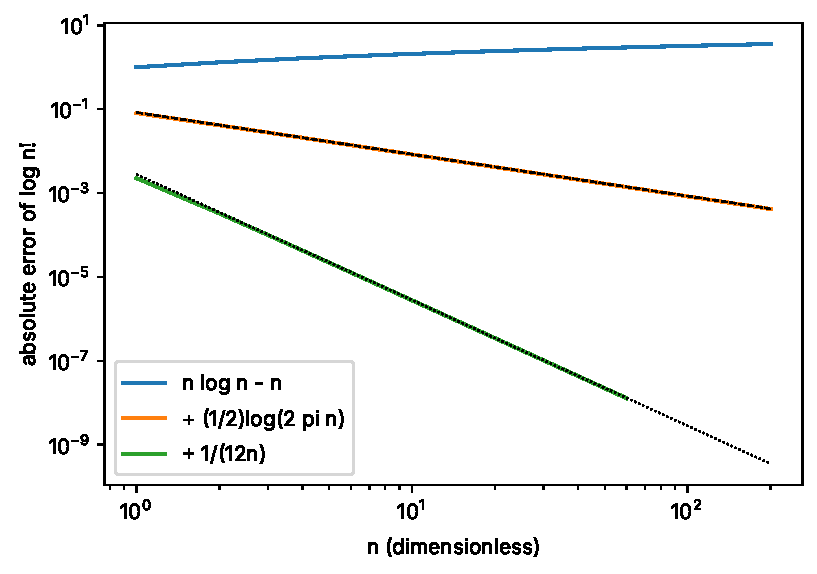
\includegraphics[width=0.85\linewidth]{figs/asymptotics_stirling.pdf}
\caption{Absolute error of three truncations of Stirling's series for $\log n!$, for $1\le n\le200$ (both axes logarithmic, dimensionless). The leading term $n\log n-n$ has an error growing like $\tfrac12\log(2\pi n)$; adding $\tfrac12\log(2\pi n)$ leaves an error close to $1/(12n)$ (dashed); adding $1/(12n)$ leaves an error close to $1/(360n^3)$ (dotted).}
\label{fig:asymptotics-stirling}
\end{figure}

\begin{beyond}
\textbf{Asymptotic, not convergent.} If you continue the Stirling series \cref{eq:asymptotics-stirling-series} forever, it diverges for every $n$: the coefficients eventually grow factorially, faster than any geometric sequence $c^k$, so for every fixed $n$ the terms eventually increase. Each fixed truncation is still an excellent approximation for large $n$, and the error is smallest if you stop near the smallest term. This is a proved theorem whose proof is beyond this book; see \cite{edwards} and \cite{rhb}.
\end{beyond}

\subsection{The Gamma function}

Factorials are defined only for whole numbers. Chapter~\ref{ch:counting-zeros} needs a ``factorial'' of a complex number, and the Gamma function provides it.

\paragraph{Definition.} For real $x>0$,
\begin{equation}
\Gamma(x)=\int_0^\infty u^{x-1}e^{-u}\,\dd u .
\label{eq:asymptotics-gamma}
\end{equation}
The integral converges: near $u=0$ the integrand behaves like $u^{x-1}$, whose integral $\int_0^1u^{x-1}\dd u=1/x$ is finite for $x>0$; for large $u$, pick an integer $k\ge x+2$. For $u>0$ every term of the Taylor series of $e^u$ is positive, so $e^u>u^k/k!$. Hence $u^{x+1}e^{-u}<k!\,u^{x+1-k}\le k!/u$ for $u\ge1$, which tends to $0$. The integrand $u^{x-1}e^{-u}=u^{-2}\cdot u^{x+1}e^{-u}$ is therefore below $u^{-2}$ once $u$ is large enough, and $\int_1^\infty u^{-2}\,\dd u=1$ is finite. (This is the precise meaning of ``exponentials beat powers'' used below.)

\paragraph{The factorial property.} First, $\Gamma(1)=\int_0^\infty e^{-u}\dd u=1$. Next, integrate by parts with ``$f=u^{x}$, $\dd g=e^{-u}\dd u$'':
\[
\Gamma(x+1)=\int_0^\infty u^{x}e^{-u}\dd u=\Bigl[-u^{x}e^{-u}\Bigr]_0^\infty+\int_0^\infty xu^{x-1}e^{-u}\dd u .
\]
The bracket vanishes at both ends (at $0$ because $u^x\to0$ for $x>0$; at $\infty$ because exponentials beat powers), leaving
\begin{equation}
\Gamma(x+1)=x\,\Gamma(x).
\label{eq:asymptotics-gamma-rec}
\end{equation}
Applying this repeatedly, $\Gamma(n+1)=n\Gamma(n)=n(n-1)\Gamma(n-1)=\dots=n!\,\Gamma(1)=n!$. So $\Gamma$ is a smooth function that passes through the factorials, shifted by one: $\Gamma(n+1)=n!$. A half-integer value: substituting $u=y^2$ in \cref{eq:asymptotics-gamma} gives $\Gamma(\tfrac12)=2\int_0^\infty e^{-y^2}\dd y=\sqrt\pi=1.772454$, using the Gaussian integral (taken on trust, as in the box above).

\paragraph{Stirling for the Gamma function.} Since $\log\Gamma(n)=\log n!-\log n$, \cref{eq:asymptotics-stirling-series} gives $\log\Gamma(n)=(n-\tfrac12)\log n-n+\tfrac12\log2\pi+\tfrac1{12n}-\cdots$. That the same expansion holds for real $x$, not only for integers, is the content of the following box.
\begin{beyond}
\textbf{Stirling for real arguments.} The expansion \cref{eq:asymptotics-stirling-gamma} below holds as $x\to\infty$ through all real values, not only through the integers where we derived it. This is a proved result whose proof (by the Euler--Maclaurin summation formula applied to $\log\Gamma$) is beyond this book; see \cite{rhb}. We take it on trust.
\end{beyond}
\noindent Taken on trust as stated in the box,
\begin{equation}
\log\Gamma(x)=\Bigl(x-\tfrac12\Bigr)\log x-x+\tfrac12\log2\pi+\frac{1}{12x}-\frac{1}{360x^3}+\order(x^{-5}),\quad x\to\infty .
\label{eq:asymptotics-stirling-gamma}
\end{equation}
For example at $x=5$, $\log\Gamma(5)=\log24=3.178054$; the formula through $1/(12x)$ gives $3.178076$, and with the $-1/(360x^3)$ term it gives $3.178054$.

\begin{beyond}
\textbf{Stirling for complex arguments.} The Gamma function extends to complex $z$ (except $z=0,-1,-2,\dots$), and \cref{eq:asymptotics-stirling-gamma} remains true with $x$ replaced by complex $z$:
\[
\log\Gamma(z)=\Bigl(z-\tfrac12\Bigr)\log z-z+\tfrac12\log2\pi+\frac{1}{12z}+\order(\abs{z}^{-3}),
\]
as $\abs{z}\to\infty$ in any sector $\abs{\arg z}\le\pi-\delta$ with $\delta>0$ fixed. Here $\log z$ is the principal branch (Chapter~\ref{ch:complex}), and $\log\Gamma(z)$ is the branch that is real on the positive real axis and continuous away from the negative real axis. Proofs are in \cite{edwards} and \cite{titchmarsh}. We use this only as a tool.
\end{beyond}

\paragraph{Preview: where the $\tfrac78$ comes from.} Chapter~\ref{ch:counting-zeros} introduces the Riemann--Siegel theta function $\theta(t)=\arg\Gamma(\tfrac14+\tfrac{it}{2})-\tfrac t2\log\pi$ and uses the complex Stirling formula with $z=\tfrac14+\tfrac{it}2$ to derive
\begin{equation}
\theta(t)=\frac t2\log\frac{t}{2\pi}-\frac t2-\frac\pi8+\frac{1}{48t}+\order(t^{-3}).
\label{eq:asymptotics-theta}
\end{equation}
That chapter also shows the counting function is $N(t)=\theta(t)/\pi+1+S(t)$. Dropping $S$ and the $1/(48t)$ term, $\theta/\pi+1=\frac{t}{2\pi}\log\frac{t}{2\pi}-\frac{t}{2\pi}-\frac18+1$, which is exactly \cref{eq:asymptotics-nsm} with $-\tfrac18+1=\tfrac78$. You can check \cref{eq:asymptotics-theta} numerically with \texttt{mpmath.siegeltheta}: at $t=100$ it returns $87.97216$, while the first three terms give $87.97196$, a difference of $2.08\times10^{-4}$, which is $1/(48t)$ to within $10^{-8}$.

\begin{checkpoint}
Why does Stirling's formula \cref{eq:asymptotics-stirling} contain $\tfrac12\log(2\pi n)$ while the crude bounds \cref{eq:asymptotics-lognfact-bounds} only bracket the error between $1$ and $1+\log n$?
\end{checkpoint}
\checkanswer{The bounds treat each rectangle as entirely above or below the curve. For a slowly curving function the true sum is close to the average of the two, which accounts for the $\tfrac12\log n$ (half of $\log n$). The remaining constant $\tfrac12\log2\pi$ comes from the exact limit $C$, which crude bounds cannot see.}

\begin{keyideas}
\item Stirling: $\log n!=n\log n-n+\tfrac12\log(2\pi n)+\vartheta_n/(12n)$ with $0<\vartheta_n<1$, \cref{eq:asymptotics-stirling}; the bound on $\vartheta_n$ was proved here, the constant $\tfrac12\log2\pi$ taken on trust.
\item $\Gamma(x)=\int_0^\infty u^{x-1}e^{-u}\dd u$, $\Gamma(x+1)=x\Gamma(x)$, $\Gamma(n+1)=n!$.
\item Stirling extends to $\log\Gamma$ for real and (beyond this book) complex arguments; this is the origin of the $\tfrac78$ in the paper's Eq.~(1).
\end{keyideas}

%======================================================================
\section{Inverting a monotone function}\label{sec:asymptotics-inverse}

The paper defines the smooth zeros implicitly: $s_n$ is the number with $\Nsm(s_n)=n-\tfrac12$ (Sec.~II~A). In the same way, Eq.~(2) gives $x$ as a function of $V$, and the solver needs $V$ as a function of $x$. Both are inversions of a monotone function.

\subsection{Existence, uniqueness and the derivative of the inverse}

\begin{beyond}
\textbf{The intermediate value theorem.} If $f$ is continuous on $[a,b]$ and $y$ lies between $f(a)$ and $f(b)$, then there is at least one $c\in[a,b]$ with $f(c)=y$. In particular, if $f(a)$ and $f(b)$ have opposite signs, $f$ has a root in $[a,b]$. This is proved in any course on real analysis; we take it on trust.
\end{beyond}

\paragraph{Theorem (inverse of a strictly increasing function).} Let $f$ be continuous and strictly increasing on an interval $I$. Then for every $y$ such that $f(a)<y<f(b)$ for some points $a<b$ of $I$, there is exactly one $x\in I$ with $f(x)=y$. We write $x=f^{-1}(y)$.

\emph{Proof.} Existence: with such $a<b$, apply the intermediate value theorem to $f$ on $[a,b]$. Uniqueness: if $x_1<x_2$ then $f(x_1)<f(x_2)$, so two different points cannot give the same value. \hfill$\square$

\paragraph{Derivative of the inverse.} Write $g=f^{-1}$, so $g(f(x))=x$ for all $x\in I$. If $f$ is differentiable with $f'(x)\neq0$, then $g$ is differentiable at $y=f(x)$ (a fact from calculus that we accept), and differentiating $g(f(x))=x$ with the chain rule gives $g'(f(x))\,f'(x)=1$, that is,
\begin{equation}
\frac{\dd x}{\dd y}=\frac{1}{\dd y/\dd x}.
\label{eq:asymptotics-inverse-derivative}
\end{equation}

\subsection{The smooth counting function is invertible for $t>2\pi$}

Differentiate \cref{eq:asymptotics-nsm} term by term. By the product rule,
\[
\frac{\dd}{\dd t}\Bigl[\frac{t}{2\pi}\log\frac{t}{2\pi}\Bigr]=\frac{1}{2\pi}\log\frac{t}{2\pi}+\frac{t}{2\pi}\cdot\frac{1}{t}=\frac{1}{2\pi}\log\frac{t}{2\pi}+\frac{1}{2\pi}.
\]
(The derivative of $\log(t/2\pi)=\log t-\log2\pi$ is $1/t$.) The second term contributes $-1/(2\pi)$ and the constant contributes $0$. The $\pm1/(2\pi)$ cancel:
\begin{equation}
\Nsm'(t)=\frac{1}{2\pi}\log\frac{t}{2\pi},\qquad \Nsm''(t)=\frac{1}{2\pi t}.
\label{eq:asymptotics-nsm-derivs}
\end{equation}
So $\Nsm'$ is negative for $t<2\pi$, zero at $t=2\pi$, and positive for $t>2\pi$; and $\Nsm''>0$ for all $t>0$ ($\Nsm$ is \emph{convex}). Convexity in this sense means that the graph lies above every tangent line: by Taylor's theorem with remainder (box in \cref{sec:asymptotics-newton}), $f(r)=f(x)+f'(x)(r-x)+\tfrac12f''(\xi)(r-x)^2\ge f(x)+f'(x)(r-x)$ whenever $f''>0$. The minimum value is $\Nsm(2\pi)=1\cdot0-1+\tfrac78=-\tfrac18$. As $t\to0^+$, $t\log t\to0$ (substitute $t=e^{-u}$ and use exponentials beat powers), so $\Nsm\to\tfrac78$. As $t\to\infty$, $\Nsm\to\infty$.

By the theorem, on $(2\pi,\infty)$ the function $\Nsm$ takes every value above $-\tfrac18$ exactly once. (Given $y>-\tfrac18$, continuity lets us take $a$ slightly above $2\pi$ with $\Nsm(a)<y$, because $\Nsm(2\pi)=-\tfrac18<y$, and $b$ large with $\Nsm(b)>y$, because $\Nsm\to\infty$.) Every $n-\tfrac12$ with $n\ge1$ is at least $\tfrac12>-\tfrac18$, so each smooth zero $s_n>2\pi$ exists and is unique. \Cref{fig:asymptotics-nsm} shows the picture.

\begin{figure}[htbp]\centering
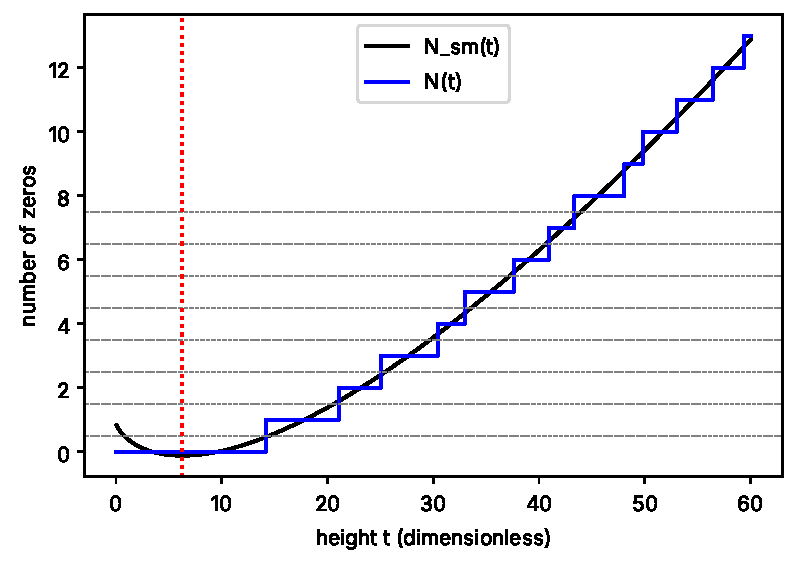
\includegraphics[width=0.85\linewidth]{figs/asymptotics_nsm.pdf}
\caption{The smooth counting function $\Nsm(t)$ of the paper's Eq.~(1) (solid) and the true zero-counting staircase $N(t)$ (steps at the zeros $t_n$), for $0<t\le60$. Dashed horizontal lines are the levels $n-\tfrac12$; the smooth zeros $s_n$ are where $\Nsm$ crosses them for $t>2\pi$. $\Nsm$ has its minimum $-\tfrac18$ at $t=2\pi$ and tends to $\tfrac78$ as $t\to0$, so the level $\tfrac12$ is crossed twice: at $s_1=14.521$ and at a spurious point $t=0.756$. The horizontal axis is the height $t$ (dimensionless); the vertical axis counts zeros.}
\label{fig:asymptotics-nsm}
\end{figure}

\begin{pitfall}
Because $\Nsm(t)\to\tfrac78$ as $t\to0$, the equation $\Nsm(t)=\tfrac12$ has a \emph{second} root, near $t=0.756$, on the decreasing branch $t<2\pi$. It has nothing to do with the zeta zeros. A root finder started carelessly at small $t$ can return it. Always restrict the search to $t>2\pi$.
\end{pitfall}

\subsection{The mean spacing}

Treat $n$ as a continuous variable and differentiate $\Nsm(s_n)=n-\tfrac12$ with respect to $n$: by the chain rule $\Nsm'(s_n)\,\frac{\dd s_n}{\dd n}=1$, which is \cref{eq:asymptotics-inverse-derivative}. With \cref{eq:asymptotics-nsm-derivs},
\begin{equation}
\gap_n=\frac{\dd s_n}{\dd n}=\frac{1}{\Nsm'(s_n)}=\frac{2\pi}{\log(s_n/2\pi)}.
\label{eq:asymptotics-gap}
\end{equation}
This is the ``local mean spacing'' in which the paper measures all errors. It shrinks slowly with height (Chapter~\ref{ch:counting-zeros} develops this in detail).

\subsection{The Lambert $W$ function}

Some inverses are important enough to have names. The \emph{Lambert $W$ function} is the inverse of $w\mapsto we^{w}$:
\begin{equation}
W(z)\,e^{W(z)}=z .
\label{eq:asymptotics-lambertw}
\end{equation}
The function $f(w)=we^w$ has $f'(w)=(1+w)e^w$, which is negative for $w<-1$ and positive for $w>-1$, so $f$ has a minimum $f(-1)=-1/e$. For $w<0$, $f(w)<0$; for $w\ge0$, $f$ increases from $0$ to $\infty$. Consequently:
\begin{itemize}
\item for $z\ge0$ there is exactly one real solution $W(z)\ge0$ (for example $W(0)=0$, $W(e)=1$);
\item for $-1/e<z<0$ there are two real solutions: the \emph{principal branch} $W_0(z)\in(-1,0)$ and the \emph{lower branch} $W_{-1}(z)<-1$;
\item for $z<-1/e$ there is no real solution.
\end{itemize}
In Python, \texttt{scipy.special.lambertw(z, k)} returns branch $k$ ($k=0$ by default, or $k=-1$); take the real part of its complex output.

\paragraph{Solving $x\log x=y$.} Put $x=e^u$. Then $x\log x=ue^u=y$, so $u=W(y)$ and $x=e^{W(y)}$. From \cref{eq:asymptotics-lambertw}, $e^{W(y)}=y/W(y)$, so
\begin{equation}
x\log x=y\quad\Longleftrightarrow\quad x=\frac{y}{W(y)}.
\label{eq:asymptotics-xlogx}
\end{equation}

\paragraph{The smooth zeros in closed form.} Combine the first two terms of \cref{eq:asymptotics-nsm}: $\frac{t}{2\pi}\bigl(\log\frac{t}{2\pi}-1\bigr)=\frac{t}{2\pi}\log\frac{t}{2\pi e}$, because $\log e=1$. So $\Nsm(s)=n-\tfrac12$ becomes
\[
\frac{s}{2\pi}\log\frac{s}{2\pi e}=n-\frac12-\frac78=n-\frac{11}{8}.
\]
Let $v=s/(2\pi e)$, so $s/(2\pi)=ev$. Then $ev\log v=n-\tfrac{11}8$, i.e. $v\log v=y_n$ with $y_n=(n-\tfrac{11}{8})/e$. By \cref{eq:asymptotics-xlogx}, $v=y_n/W(y_n)$, and $s_n=2\pi e\,v=2\pi e\,y_n/W(y_n)$:
\begin{equation}
s_n=\frac{2\pi\,(n-\frac{11}{8})}{W\!\bigl((n-\frac{11}{8})/e\bigr)} .
\label{eq:asymptotics-sn-lambert}
\end{equation}
Moreover $v=e^{W(y_n)}$ means $\log(s_n/2\pi)=\log(ev)=1+W(y_n)$, so \cref{eq:asymptotics-gap} becomes
\begin{equation}
\gap_n=\frac{2\pi}{1+W\bigl((n-\frac{11}{8})/e\bigr)} .
\label{eq:asymptotics-gap-lambert}
\end{equation}
This is the ``Lambert-$W$ asymptotic of the counting function'' that the paper mentions in Sec.~I~A in connection with Fran\c ca and LeClair \cite{francaleclair}.

\begin{sample}{The first smooth zero and its impostor}
Use \cref{eq:asymptotics-sn-lambert} for $n=1$ and explain which branch of $W$ to use.

\textbf{Step 1:} $n-\tfrac{11}8=-\tfrac38$, so $y_1=-\tfrac{3}{8e}=-0.137954$. This lies in $(-1/e,0)=(-0.3679,0)$, so there are two real values of $W$.

\textbf{Step 2:} Principal branch: $W_0(-0.137954)=-0.16226$. Then $s=2\pi(-0.375)/(-0.16226)=2.356194/0.16226=14.521$.

\textbf{Step 3:} Lower branch: $W_{-1}(-0.137954)=-3.118$, giving $s=2.356194/3.118=0.756$.

\textbf{Step 4:} Decide. By \cref{eq:asymptotics-gap-lambert}'s derivation, $\log(s/2\pi)=1+W$. The physical branch has $s>2\pi$, i.e. $1+W>0$, i.e. $W>-1$: the principal branch. The lower branch gives $s<2\pi$, the spurious root of the pitfall above.

\[
\boxed{s_1=14.521\ (W_0),\qquad \text{spurious root }0.756\ (W_{-1})}
\]
The mean spacing there is $\gap_1=2\pi/(1-0.16226)=7.500$. For $n\ge2$, $y_n>0$ and only one real branch exists, so there is no ambiguity.
\end{sample}

\begin{sample}{The thousandth zero in mean spacings}
The paper gives $t_{1000}=1419.42248094599$ (Sec.~II~A). Find $s_{1000}$, $\gap_{1000}$ and the fluctuation $(t_{1000}-s_{1000})/\gap_{1000}$.

\textbf{Step 1:} $y=(1000-\tfrac{11}{8})/e=998.625/2.718282=367.374$. Solving $we^w=367.374$ gives $W=4.4202$.

\textbf{Step 2:} By \cref{eq:asymptotics-sn-lambert}, $s_{1000}=2\pi\times998.625/4.4202=6274.546/4.4202=1419.52$. Here $W$ must be carried to five significant digits: with the rounded value $W=4.420$ the same division gives $1419.58$, and Step 4 would come out as $-0.14$ instead of $-0.08$. The fluctuation $t-s$ is a small difference of two large numbers, so it magnifies small relative errors in $s$ (the cancellation effect of \cref{sec:asymptotics-float}).

\textbf{Step 3:} By \cref{eq:asymptotics-gap-lambert}, $\gap_{1000}=2\pi/5.420=1.159$.

\textbf{Step 4:} $(1419.422-1419.52)/1.159=-0.08$.

\[
\boxed{s_{1000}=1419.52,\quad\gap_{1000}=1.159,\quad\text{fluctuation}\approx-0.08\ \text{spacings}}
\]
The true zero sits about a twelfth of a spacing below its smooth position. The paper's null rms of $0.263$ (Sec.~II~C) is the typical size of such fluctuations on zeros 401--500.
\end{sample}

\paragraph{How good is the leading order?} For large $y$, $W(y)\sim\log y$ (take logarithms of \cref{eq:asymptotics-lambertw}: $\log W+W=\log y$, and $\log W=o(W)$ by \cref{eq:asymptotics-logpower}). Hence $s_n\sim2\pi n/\log n$ and $\gap_n\sim2\pi/\log n$. But at $n=1000$, $2\pi n/\log n=909.6$, far from $s_{1000}=1419.52$, and $2\pi/\log n=0.9096$, far from $1.159$. \Cref{fig:asymptotics-lambertw} shows how slowly these ratios approach 1. The lesson of \cref{sec:asymptotics-order} repeats: with logarithms, use the exact inverse, not its leading term.

\begin{figure}[htbp]\centering
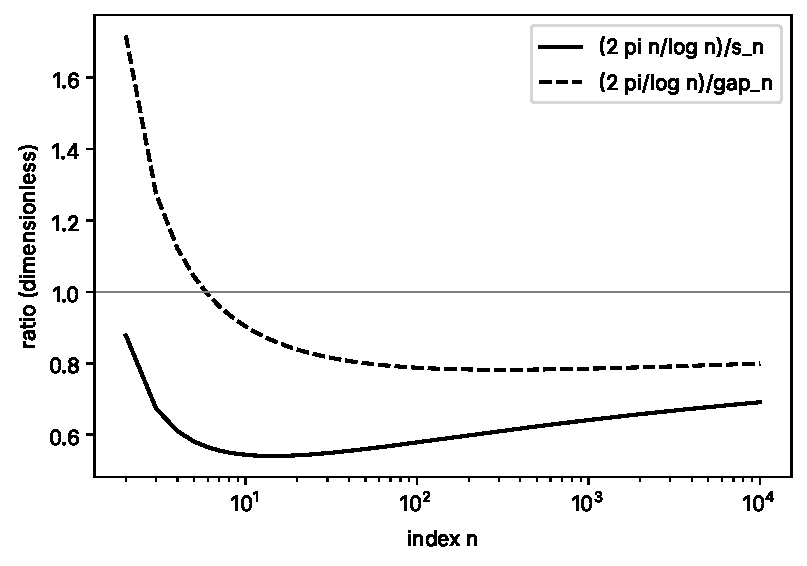
\includegraphics[width=0.85\linewidth]{figs/asymptotics_lambertw.pdf}
\caption{Ratios of leading-order approximations to exact values for the smooth zeros, $2\le n\le10^4$ (logarithmic horizontal axis, dimensionless). Solid: $(2\pi n/\log n)/s_n$; dashed: $(2\pi/\log n)/\gap_n$. Both tend to 1 as $n\to\infty$, but at $n=10^4$ they are still far from it. The exact values come from the Lambert-$W$ formulas \cref{eq:asymptotics-sn-lambert,eq:asymptotics-gap-lambert}.}
\label{fig:asymptotics-lambertw}
\end{figure}

\paragraph{Numerical inversion in general.} Most monotone functions have no named inverse. Eq.~(2) of the paper, which gives the Wu--Sprung position $x(V)$, is such a case; the paper says it is ``inverted pointwise by bracketed root finding'' (Sec.~II~B). The general recipe for computing $f^{-1}(y)$ is: (i) find an interval $[a,b]$ with $f(a)<y<f(b)$; (ii) solve $f(x)-y=0$ in it with a root finder. The rest of this chapter is about step (ii).

\begin{checkpoint}
The Lambert-$W$ formula gives every smooth zero in one line. Why might a program still use a root finder for $s_n$?
\end{checkpoint}
\checkanswer{Because a root finder works for any continuous function with a sign change, including the Wu--Sprung inversion and the level equations $\Nsm(t)+\Nfl(t)=n-\tfrac12$ used later ($\Nfl$ is an oscillating prime sum, Chapter~\ref{ch:explicit-formula}), which need not even be monotone and have no closed form. Using one tool for all of them is simpler and lets you cross-check against the closed form where it exists.}

\begin{keyideas}
\item A continuous strictly increasing function has a unique inverse; $\dd x/\dd y=1/(\dd y/\dd x)$, \cref{eq:asymptotics-inverse-derivative}.
\item $\Nsm'(t)=\frac{1}{2\pi}\log\frac{t}{2\pi}$, so $\Nsm$ is increasing for $t>2\pi$ and each $s_n$ is unique there; $\gap_n=2\pi/\log(s_n/2\pi)$, \cref{eq:asymptotics-gap}.
\item $s_n=2\pi(n-\frac{11}8)/W((n-\frac{11}8)/e)$ with the principal branch, \cref{eq:asymptotics-sn-lambert}; the other branch gives a spurious root.
\end{keyideas}

%======================================================================
\section{Root finding I: bisection}\label{sec:asymptotics-bisection}
% DYK-BEGIN
\begin{didyouknow}{A Theorem Behind Bisection}
Bisection works because a continuous function that changes sign must cross zero somewhere in between. That sounds obvious, but Bernard Bolzano gave one of the first rigorous proofs only in 1817. Each bisection step halves the interval, so ten steps shrink it by a factor $2^{10}=1024$, gaining about three decimal digits. The method is slow, but once a sign change is bracketed it never fails.
\end{didyouknow}
% DYK-END

A \emph{root} of a function $f$ is a number $r$ with $f(r)=0$. To compute $s_n$ we find the root of $f(s)=\Nsm(s)-(n-\tfrac12)$. The simplest reliable method is to trap the root in an interval and keep halving it.

\subsection{The algorithm}

Suppose $f$ is continuous on $[a,b]$ and $f(a)$, $f(b)$ have opposite signs; we call $[a,b]$ a \emph{bracket}. By the intermediate value theorem the bracket contains a root.
\begin{enumerate}
\item Compute the midpoint $m=(a+b)/2$ and $f(m)$.
\item If $f(a)$ and $f(m)$ have opposite signs (or $f(m)=0$), the new bracket is $[a,m]$; otherwise it is $[m,b]$.
\item Repeat until the bracket is short enough; return its midpoint.
\end{enumerate}
In step 2, if $f(a)f(m)>0$ then $f(m)$ has the sign of $f(a)$, which is opposite to the sign of $f(b)$, so $[m,b]$ is a bracket. Either way the new interval is a bracket.

\subsection{A guaranteed error bound}

Let $[a_k,b_k]$ be the bracket after $k$ halvings, with $[a_0,b_0]=[a,b]$. Each step halves the width, so $b_k-a_k=(b-a)/2^k$. The root $r$ lies in $[a_k,b_k]$, and the midpoint $m_k=(a_k+b_k)/2$ is at most half the width from any point of the bracket:
\begin{equation}
\abs{m_k-r}\le\frac{b-a}{2^{k+1}} .
\label{eq:asymptotics-bisect-bound}
\end{equation}
To guarantee $\abs{m_k-r}\le\delta$ we need $2^{k+1}\ge(b-a)/\delta$, that is,
\begin{equation}
k\ge\log_2\frac{b-a}{\delta}-1 .
\label{eq:asymptotics-bisect-steps}
\end{equation}
Each step costs one function evaluation and gains one binary digit, about $0.3$ decimal digits. The bound holds whatever $f$ looks like, provided it is continuous: that is the great virtue of bisection.

\begin{sample}{Bisection for the first smooth zero}
Find $s_1$ by bisection on $f(s)=\Nsm(s)-\tfrac12$, starting from $[10,20]$. Do five steps and determine how many steps would guarantee an error below $10^{-10}$.

\textbf{Step 1:} Check the bracket: $f(10)=-0.4769$ and $f(20)=0.8775$ have opposite signs. Both points exceed $2\pi\approx6.28$, where $f$ is increasing, so the bracket contains exactly one root.

\textbf{Step 2:} Iterate. Each row shows the midpoint, the sign of $f$ there, and the new bracket:
\begin{center}
\begin{tabular}{cccc}
\toprule
$k$ & midpoint $m$ & $f(m)$ & new bracket\\
\midrule
1 & 15 & $+0.0651$ & $[10,15]$\\
2 & 12.5 & $-0.2460$ & $[12.5,15]$\\
3 & 13.75 & $-0.0995$ & $[13.75,15]$\\
4 & 14.375 & $-0.0194$ & $[14.375,15]$\\
5 & 14.6875 & $+0.0223$ & $[14.375,14.6875]$\\
\bottomrule
\end{tabular}
\end{center}

\textbf{Step 3:} After five steps the width is $10/2^5=0.3125$; the midpoint $14.53125$ has guaranteed error at most $0.15625$ by \cref{eq:asymptotics-bisect-bound}. The actual error, using the converged root $s_1=14.5213$ (found with Brent's method, \cref{sec:asymptotics-newton}), is about $0.0099$.

\textbf{Step 4:} For $\delta=10^{-10}$, \cref{eq:asymptotics-bisect-steps} requires $k\ge\log_2(10^{11})-1=36.54-1=35.54$, so $k=36$.

\[
\boxed{s_1\in[14.375,\,14.6875]\text{ after 5 steps};\quad 36\text{ steps for }10^{-10}}
\]
\end{sample}

\begin{pycode}
import numpy as np

def Nsm(t):                          # paper Eq. (1)
    u = t / (2 * np.pi)
    return u * np.log(u) - u + 7 / 8

def bisect(f, a, b, tol):
    fa, fb = f(a), f(b)
    if fa * fb > 0:
        raise ValueError("f(a) and f(b) have the same sign")
    while (b - a) / 2 > tol:
        m = (a + b) / 2
        fm = f(m)
        if fa * fm <= 0:             # sign change in [a, m]
            b, fb = m, fm
        else:                        # sign change in [m, b]
            a, fa = m, fm
    return (a + b) / 2

s1 = bisect(lambda s: Nsm(s) - 0.5, 10.0, 20.0, 1e-10)
print(s1)                            # 14.5213...
\end{pycode}

\begin{checkpoint}
You start bisection with a bracket of width 1 and do 10 steps. What is the largest possible error of the midpoint?
\end{checkpoint}
\checkanswer{By \cref{eq:asymptotics-bisect-bound}, $1/2^{11}=4.9\times10^{-4}$.}

\begin{keyideas}
\item A bracket $[a,b]$ with $f(a)f(b)<0$ contains a root (for continuous $f$).
\item Bisection halves the bracket each step: error at most $(b-a)/2^{k+1}$ after $k$ steps, \cref{eq:asymptotics-bisect-bound}.
\item It always works but gains only one bit per evaluation.
\end{keyideas}

%======================================================================
\section{Root finding II: Newton, secant and Brent}\label{sec:asymptotics-newton}

Bisection uses only the \emph{signs} of $f$. If we also use its \emph{values}, and perhaps its slope, we can converge much faster.

\subsection{Newton's method}

Near a point $x_k$, a smooth function is close to its tangent line, $f(x)\approx f(x_k)+f'(x_k)(x-x_k)$. Set this to zero and solve for $x$; call the answer $x_{k+1}$:
\begin{equation}
x_{k+1}=x_k-\frac{f(x_k)}{f'(x_k)} .
\label{eq:asymptotics-newton}
\end{equation}
This is \emph{Newton's method}. Geometrically, follow the tangent at $(x_k,f(x_k))$ down to where it crosses the axis.

\begin{beyond}
\textbf{Taylor's theorem with remainder.} If $f$ has a continuous second derivative between $x$ and $r$, then
$f(r)=f(x)+f'(x)(r-x)+\tfrac12f''(\xi)(r-x)^2$ for some $\xi$ between $x$ and $r$. This is a standard calculus result (it is the Taylor series of Chapter~\ref{ch:series} stopped after two terms, with an exact formula for what is left); we take it on trust.
\end{beyond}

\paragraph{Quadratic convergence.} Let $r$ be a root with $f'(r)\ne0$, and let $e_k=x_k-r$ be the error. Apply Taylor's theorem at $x=x_k$, using $f(r)=0$:
\[
0=f(x_k)+f'(x_k)(r-x_k)+\tfrac12f''(\xi_k)(r-x_k)^2 .
\]
Divide by $f'(x_k)$ and rearrange:
\[
x_k-\frac{f(x_k)}{f'(x_k)}-r=\frac{f''(\xi_k)}{2f'(x_k)}(x_k-r)^2 .
\]
The left side is $x_{k+1}-r=e_{k+1}$ by \cref{eq:asymptotics-newton}. Hence
\begin{equation}
e_{k+1}=\frac{f''(\xi_k)}{2f'(x_k)}\,e_k^2\;\approx\;\frac{f''(r)}{2f'(r)}\,e_k^2\quad\text{when }x_k\text{ is close to }r.
\label{eq:asymptotics-newton-quadratic}
\end{equation}
The error is \emph{squared} at each step: once you have a few correct digits, the number of correct digits roughly doubles per iteration.

\begin{sample}{Newton's method for $\sqrt2$ and for $s_1$}
(a) Find $\sqrt2$ as the positive root of $f(x)=x^2-2$, starting at $x_0=1$. (b) Find $s_1$ starting at $x_0=14$.

\textbf{Step 1:} For (a), $f'(x)=2x$, so \cref{eq:asymptotics-newton} gives $x_{k+1}=x_k-(x_k^2-2)/(2x_k)=\tfrac12(x_k+2/x_k)$.

\textbf{Step 2:} Iterate and record $e_k=x_k-\sqrt2$, with $\sqrt2=1.41421356237$:
\begin{center}
\begin{tabular}{ccc}
\toprule
$k$ & $x_k$ & $e_k$\\
\midrule
1 & 1.5 & $8.58\times10^{-2}$\\
2 & 1.4166667 & $2.45\times10^{-3}$\\
3 & 1.4142157 & $2.12\times10^{-6}$\\
4 & 1.41421356237 & $1.59\times10^{-12}$\\
\bottomrule
\end{tabular}
\end{center}

\textbf{Step 3:} Compare with \cref{eq:asymptotics-newton-quadratic}: $f''/(2f')=2/(4\sqrt2)=1/(2\sqrt2)$, so $e_{k+1}\approx e_k^2/2.828$. From $e_2=2.45\times10^{-3}$ this predicts $e_3\approx2.13\times10^{-6}$, and from $e_3$ it predicts $e_4\approx1.59\times10^{-12}$, in agreement with the table.

\textbf{Step 4:} For (b), $f(s)=\Nsm(s)-\tfrac12$ and $f'(s)=\frac{1}{2\pi}\log\frac{s}{2\pi}$ by \cref{eq:asymptotics-nsm-derivs}. At $x_0=14$: $f(14)=-0.0680$ and $f'(14)=0.1275$, so $x_1=14+0.0680/0.1275=14.5333$.

\textbf{Step 5:} The next iterate $x_2$ agrees with the converged root $s_1=14.5213$ to better than $2\times10^{-5}$, and $x_3$ to better than $10^{-10}$.

\[
\boxed{\sqrt2:\ 12\text{ correct digits in 4 steps};\qquad s_1=14.5213\text{ in 2 to 3 steps}}
\]
Compare: bisection needed 36 steps for $10^{-10}$.
\end{sample}

\subsection{When Newton fails, and when it cannot}

Newton's method has no bracket and no guarantee. If $f'(x_k)$ is small, the tangent is nearly flat and the step is huge. A classic failure is $f(x)=\arctan x$, whose only root is $0$. Here $f'(x)=1/(1+x^2)$, so $x_{k+1}=x_k-(1+x_k^2)\arctan x_k$. From $x_0=1.5$: $x_1=-1.694$, $x_2=2.321$, and the iterates fly off with growing magnitude (\cref{fig:asymptotics-newtonfail}). From $x_0=1$ the iteration converges.

\begin{figure}[htbp]\centering
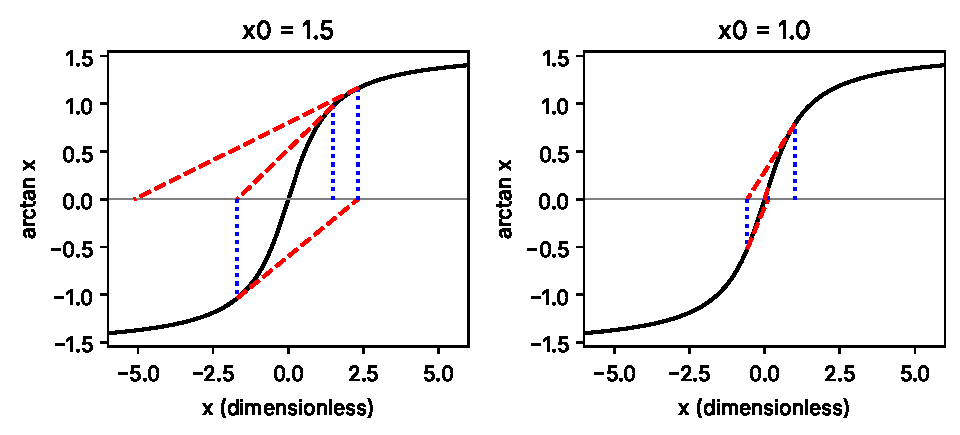
\includegraphics[width=0.85\linewidth]{figs/asymptotics_newtonfail.pdf}
\caption{Newton's method on $f(x)=\arctan x$ (dimensionless). Each dashed segment is a tangent line followed from $(x_k,f(x_k))$ to the axis. Left: from $x_0=1.5$ the iterates $-1.694$, $2.321,\ldots$ alternate in sign and grow; the method diverges. Right: from $x_0=1$ the iterates converge rapidly to the root $0$.}
\label{fig:asymptotics-newtonfail}
\end{figure}

For our problem, though, convexity rescues Newton completely.

\paragraph{Theorem (Newton on an increasing convex function).} Let $f$ be continuously differentiable, with $f'>0$ and $f$ convex on an interval $I$ ($f$ lies above all its tangent lines), and let $r\in I$ be a root. If $x_k\in I$, then $x_{k+1}\ge r$. If moreover $x_k>r$, then $r\le x_{k+1}<x_k$. Hence, as long as the iterates stay in $I$, from the first step on they decrease monotonically to $r$.

\emph{Proof.} Convexity at $x_k$, evaluated at $r$: $f(r)\ge f(x_k)+f'(x_k)(r-x_k)$. With $f(r)=0$ this is $0\ge f(x_k)-f'(x_k)(x_k-r)$, so $f(x_k)/f'(x_k)\le x_k-r$, i.e. $x_{k+1}=x_k-f(x_k)/f'(x_k)\ge r$. If $x_k>r$, then $f(x_k)>0$ (increasing $f$), so $x_{k+1}<x_k$. A decreasing sequence bounded below by $r$ converges (monotone convergence, box in \cref{sec:asymptotics-stirling}) to some $\ell$ with $r\le\ell\le x_1$, so $\ell\in I$ (an interval containing $r$ and $x_1$ contains every point between them). Since $f$ and $f'$ are continuous and $f'(\ell)>0$, the right side of \cref{eq:asymptotics-newton} converges to $\ell-f(\ell)/f'(\ell)$, while the left side converges to $\ell$. Hence $\ell=\ell-f(\ell)/f'(\ell)$, so $f(\ell)=0$, and because $f$ is increasing, $\ell=r$. \hfill$\square$

By \cref{eq:asymptotics-nsm-derivs}, $\Nsm$ is increasing and convex on $(2\pi,\infty)$. Take $I=(2\pi,\infty)$ and $r=s_n$. If $x_0\in I$, the theorem gives $x_1\ge s_n>2\pi$, so $x_1$ again lies in $I$; repeating the argument, every iterate stays in $I$, and the theorem applies at every step. So Newton's method for any smooth zero, started anywhere above $2\pi$, lands at or to the right of $s_n$ after one step and then marches down to it. (Problem~23 shows that the first step from near $2\pi$ can overshoot enormously, but it overshoots to the right, which is safe.)

\subsection{The secant method}

Newton needs $f'$. If the derivative is unavailable, replace it by the slope of the chord through the last two points:
\begin{equation}
x_{k+1}=x_k-f(x_k)\,\frac{x_k-x_{k-1}}{f(x_k)-f(x_{k-1})} .
\label{eq:asymptotics-secant}
\end{equation}
This is the \emph{secant method}. Its error satisfies $e_{k+1}\approx Ce_ke_{k-1}$, which leads to $\abs{e_{k+1}}\approx\text{const}\times\abs{e_k}^{1.618}$; the exponent is the golden ratio $(1+\sqrt5)/2$ (Problem~18 derives this). That is slower than Newton per step, but each step needs only one new function evaluation.

\paragraph{Inverse quadratic interpolation.} With three points $(a,f_a)$, $(b,f_b)$, $(c,f_c)$ with distinct $f$-values, fit $x$ as a quadratic function of $y$ through them and evaluate at $y=0$. To build that quadratic, define
\[
\ell_a(y)=\frac{(y-f_b)(y-f_c)}{(f_a-f_b)(f_a-f_c)},
\]
and $\ell_b$, $\ell_c$ in the same way with the letters cycled. Each $\ell$ is a quadratic in $y$ that equals 1 at its own $f$-value and 0 at the other two, so $x(y)=a\,\ell_a(y)+b\,\ell_b(y)+c\,\ell_c(y)$ passes through all three points (this is the \emph{Lagrange form}). Setting $y=0$ gives
\[
x_{\rm new}=\frac{a\,f_bf_c}{(f_a-f_b)(f_a-f_c)}+\frac{b\,f_af_c}{(f_b-f_a)(f_b-f_c)}+\frac{c\,f_af_b}{(f_c-f_a)(f_c-f_b)} .
\]
(Each fraction is the Lagrange basis polynomial in $y$ evaluated at $y=0$: it equals 1 when $y$ is the matching $f$-value and 0 at the other two.) Fitting $x(y)$ instead of $y(x)$ avoids solving a quadratic equation.

\subsection{Brent's method: safety plus speed}

The fast methods can wander off; bisection is slow but cannot fail. \emph{Brent's method} \cite{brent} combines them. It keeps a bracket $[b,c]$ with $f(b)f(c)<0$ at all times, with $b$ the best estimate so far, plus the previous iterate $a$. At each step:
\begin{enumerate}
\item It proposes a fast step: inverse quadratic interpolation through $a,b,c$ if their $f$-values are distinct, otherwise a secant step through $a,b$.
\item It accepts the fast step only if the new point lies well inside the bracket (between $(3c+b)/4$ and $b$) and the step is shrinking quickly enough (less than half the step before last). Otherwise it takes a bisection step instead.
\item It evaluates $f$ at the new point and updates the three points so that the bracket property is preserved.
\end{enumerate}
The result never does much worse than bisection (Brent \cite{brent} shows, and we quote without proof, that the number of evaluations never exceeds roughly $(\log_2(w_0/\delta))^2$, where $w_0$ is the width of the initial bracket and $\delta$ the requested tolerance) and on smooth functions converges superlinearly like the secant method \cite{brent,nr}. We use it as a reliable black box: \texttt{scipy.optimize.brentq(f, a, b)}. Its default tolerances are an absolute $2\times10^{-12}$ and a relative $8.88\times10^{-16}$ (four times the double-precision machine epsilon of \cref{sec:asymptotics-float}). \Cref{fig:asymptotics-convergence} compares all four methods on the first smooth zero.

\begin{figure}[htbp]\centering
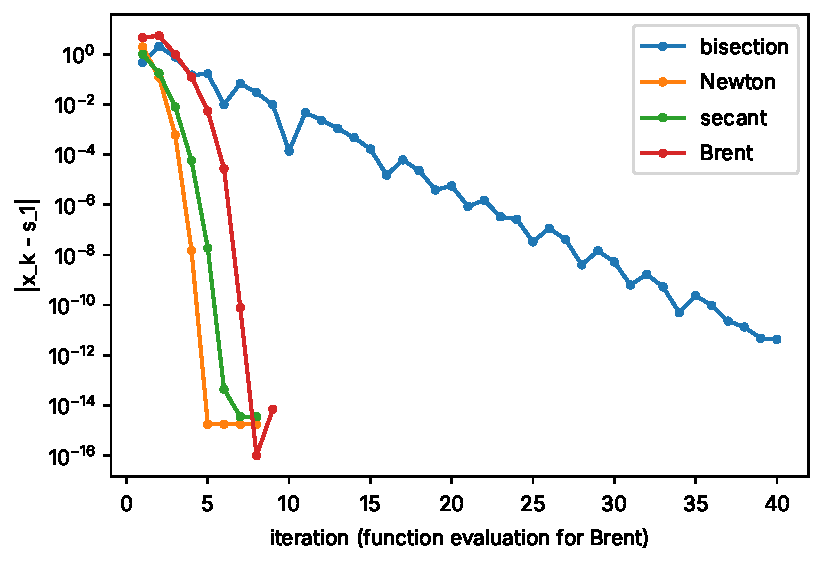
\includegraphics[width=0.85\linewidth]{figs/asymptotics_convergence.pdf}
\caption{Absolute error $\abs{x_k-s_1}$ (logarithmic) against iteration number for four root finders solving $\Nsm(s)=\tfrac12$. Bisection and Brent start from the bracket $[10,20]$; the secant method from the points $10$ and $20$; Newton from $x_0=10$. For Brent every function evaluation is plotted. Bisection gains a fixed factor of 2 per step (a straight line); Newton, secant and Brent bend downward (superlinear convergence). Errors below $10^{-16}$ are plotted at $10^{-16}$.}
\label{fig:asymptotics-convergence}
\end{figure}

\begin{pycode}
import numpy as np
from scipy.optimize import brentq

def Nsm(t):
    u = t / (2 * np.pi)
    return u * np.log(u) - u + 7 / 8

def newton(f, fprime, x, steps):
    for k in range(steps):
        x = x - f(x) / fprime(x)
    return x

n = 1
f  = lambda s: Nsm(s) - (n - 0.5)
fp = lambda s: np.log(s / (2 * np.pi)) / (2 * np.pi)

print(newton(f, fp, 14.0, 4))        # Newton
print(brentq(f, 10.0, 20.0))         # Brent on a bracket
\end{pycode}

\begin{checkpoint}
Newton's error is $10^{-3}$ at some step and $f''/(2f')\approx0.04$ near the root. Roughly what is the error after the next step? After two more?
\end{checkpoint}
\checkanswer{By \cref{eq:asymptotics-newton-quadratic}, $0.04\times(10^{-3})^2=4\times10^{-8}$, then $0.04\times(4\times10^{-8})^2\approx6\times10^{-17}$, which is below double-precision resolution.}

\begin{keyideas}
\item Newton: $x_{k+1}=x_k-f(x_k)/f'(x_k)$, error squared each step, \cref{eq:asymptotics-newton-quadratic}; can diverge in general.
\item For an increasing convex $f$ (such as $\Nsm$ on $t>2\pi$) Newton converges monotonically after one step.
\item Secant and inverse quadratic interpolation avoid derivatives; Brent's method combines them with bisection to keep a guaranteed bracket.
\end{keyideas}

%======================================================================
\section{Bracketing failures and bracket expansion}\label{sec:asymptotics-brackets}

Bisection and Brent need a bracket. Getting one is often the hardest part.

\subsection{How brackets fail}

\begin{itemize}
\item \textbf{No sign change, but roots.} If $[a,b]$ contains an even number of roots, $f(a)$ and $f(b)$ have the same sign. For example $f(t)=\Nsm(t)-\tfrac12$ is positive at both $t=0.5$ ($f=0.094$) and $t=20$ ($f=0.8775$) although it vanishes twice in between, at $0.756$ and $14.521$. A root of even multiplicity, like $x=0$ for $x^2$, never produces a sign change at all.
\item \textbf{No sign change, no root.} The obvious case: the root is outside the interval.
\item \textbf{Sign change without a root.} If $f$ is discontinuous, the intermediate value theorem does not apply. Bisection on $1/x$ over $[-1,2]$ produces midpoints $0.5,-0.25,0.125,\dots$ that converge to $0$, which is a pole, not a root. (On $[-1,1]$ it would fail at once: the first midpoint is exactly $0$, where $1/x$ cannot be evaluated.)
\item \textbf{Several roots inside.} A bracket with a sign change may contain three (or any odd number of) roots; the method returns one of them, and which one depends on details of the algorithm.
\end{itemize}

\subsection{Bracket expansion}

When a root is expected near a known guess, a standard remedy is to start from a small interval around the guess and widen it until the signs differ; for an increasing function the root found this way is the only one. The paper does exactly this for the oracle: Brent ``bracketed $\pm3$ around the smooth zero (bracket expanded on sign failure)'' (Appendix~A step 8). For the oracle a root near $s_n$ is expected, but monotonicity is not guaranteed (see the discussion of root ambiguity below). The paper does not state the units of the $\pm3$; the companion library \texttt{qmnt} uses $\pm3$ mean spacings, and so do we.

\begin{pycode}
import numpy as np
from scipy.optimize import brentq
import qmnt

def solve_level(F, n, width=3.0, grow=1.5, maxtries=20):
    """Root of Nsm(t) + F(t) = n - 1/2 near the smooth zero s_n."""
    s = qmnt.smooth_zeros(np.array([n]))[0]
    g = qmnt.mean_gap(np.array([n]))[0]
    h = lambda t: qmnt.Nsm(t) + F(t) - (n - 0.5)
    for k in range(maxtries):
        a = max(s - width * g, 2 * np.pi)   # never cross t = 2 pi
        b = s + width * g
        if h(a) * h(b) < 0:
            return brentq(h, a, b)
        width *= grow                      # widen and try again
    raise RuntimeError("no sign change found")

# with F = 0 this reproduces the smooth zero itself
print(solve_level(lambda t: 0.0, 1))       # 14.5213...
\end{pycode}

\begin{sample}{A safe bracket for $s_1$}
Find a bracket for $f(t)=\Nsm(t)-\tfrac12$ that is guaranteed to contain $s_1$ and nothing else.

\textbf{Step 1:} The naive choice $[0.5,20]$ fails: $f(0.5)=0.094>0$ and $f(20)=0.8775>0$.

\textbf{Step 2:} Use the structure from \cref{sec:asymptotics-inverse}: on $[2\pi,\infty)$, $f$ is strictly increasing. At the left end, $f(2\pi)=-\tfrac18-\tfrac12=-0.625<0$.

\textbf{Step 3:} At the right end, $f(20)=0.8775>0$.

\[
\boxed{[2\pi,\,20]\text{ brackets exactly one root, }s_1=14.521}
\]
The lesson: use what you know about the function (here, monotonicity on a half-line) to choose brackets. Blind brackets can trap the wrong root or none.
\end{sample}

\subsection{Root ambiguity}

Adding an oscillating term to $\Nsm$ can destroy monotonicity. The level equation of the paper's oracle is $\Nsm(t)+\Nfl(t)=n-\tfrac12$ (Sec.~II~D), where $\Nfl$ is a sum of sines (Chapter~\ref{ch:explicit-formula}). The left side is increasing as long as $\abs{\Nfl'(t)}<\Nsm'(t)$. If the oscillation is steep enough to violate this, the left side can wiggle back down and the equation can have three roots near one level. Then ``the'' predicted zero is ambiguous, and different brackets give different answers. The same can happen for the paper's fitted controls, whose level equation is $\Nsm(t)+F(t)=n-\tfrac12$ with a fitted sum of sinusoids $F$: Table~IV flags the control-B row with 900 fitted coefficients as root-ambiguous (Sec.~IV). Problem~30 explores the monotonicity condition for the oracle, and Chapter~\ref{ch:sparse-frequency} treats the ambiguity in detail.

\begin{checkpoint}
Why can bisection not find the root of $f(x)=x^2$?
\end{checkpoint}
\checkanswer{$x^2\ge0$ everywhere, so no interval gives a sign change; bisection needs $f(a)f(b)<0$. A double root touches the axis without crossing it.}

\begin{keyideas}
\item A bracket needs a sign change of a \emph{continuous} function; even numbers of roots, double roots and poles defeat it.
\item Use known monotonicity to choose brackets; expand them systematically when the sign test fails (paper, Appendix~A step 8).
\item Non-monotone level equations can have several roots: a root finder then returns one of them, not ``the'' answer.
\end{keyideas}

%======================================================================
\section{Floating-point numbers}\label{sec:asymptotics-float}

A computer cannot store $\pi$ or even $0.1$ exactly. It stores a nearby \emph{floating-point number}, and every arithmetic operation rounds its result. Usually this is harmless. Sometimes, as in Sec.~V of the paper, it is not.

\subsection{Binary scientific notation}

A floating-point number is stored as
\begin{equation}
x=\pm\,(1.b_1b_2\ldots b_p)_2\times2^{e},
\label{eq:asymptotics-float}
\end{equation}
where each $b_i$ is a binary digit (0 or 1), $(1.b_1\ldots b_p)_2=1+b_1/2+b_2/4+\dots+b_p/2^p$, and $e$ is an integer exponent. The leading 1 is not stored (it is implied), so there are $p+1$ significant binary digits. The two formats that matter here are summarized in \cref{tab:asymptotics-formats}.

\begin{table}[htbp]\centering
\caption{The two IEEE floating-point formats used in scientific computing. ``Digits'' is $(p+1)\log_{10}2$, the number of decimal digits the significand can hold.}
\label{tab:asymptotics-formats}
\begin{tabular}{lcccccc}
\toprule
format & bits & exponent bits & $p$ & machine epsilon $2^{-p}$ & digits & largest value\\
\midrule
double (float64) & 64 & 11 & 52 & $2.22\times10^{-16}$ & 15.95 & $1.80\times10^{308}$\\
single (float32) & 32 & 8 & 23 & $1.19\times10^{-7}$ & 7.22 & $3.40\times10^{38}$\\
\bottomrule
\end{tabular}
\end{table}

Some numbers are exact: $10=(1.01)_2\times2^3$. Others are not: $0.1=(1.100110011\ldots)_2\times2^{-4}$ repeats forever in binary, just as $1/3$ repeats in decimal, so it must be rounded.

\paragraph{Machine epsilon.} The \emph{machine epsilon} $\varepsilon$ is the gap between 1 and the next larger floating-point number. From \cref{eq:asymptotics-float}, the next number after $(1.00\ldots0)_2$ is $(1.00\ldots01)_2=1+2^{-p}$, so $\varepsilon=2^{-p}$: $2.22\times10^{-16}$ in double and $1.19\times10^{-7}$ in float32.

\paragraph{The rounding model.} Rounding to the nearest floating-point number moves $x$ by at most half the local spacing. Near $2^e$ the spacing is $\varepsilon\,2^e$, and $\abs{x}\ge2^e$, so the relative error is at most $\varepsilon/2$:
\begin{equation}
\mathrm{fl}(x)=x(1+\delta),\qquad\abs{\delta}\le\frac{\varepsilon}{2}.
\label{eq:asymptotics-roundmodel}
\end{equation}
The same holds for each $+$, $-$, $\times$, $\div$: the computer returns the exact result of the operation on the stored numbers, rounded by \cref{eq:asymptotics-roundmodel}. \Cref{fig:asymptotics-float} shows the relative rounding error of float32 across several powers of 2.

\begin{figure}[htbp]\centering
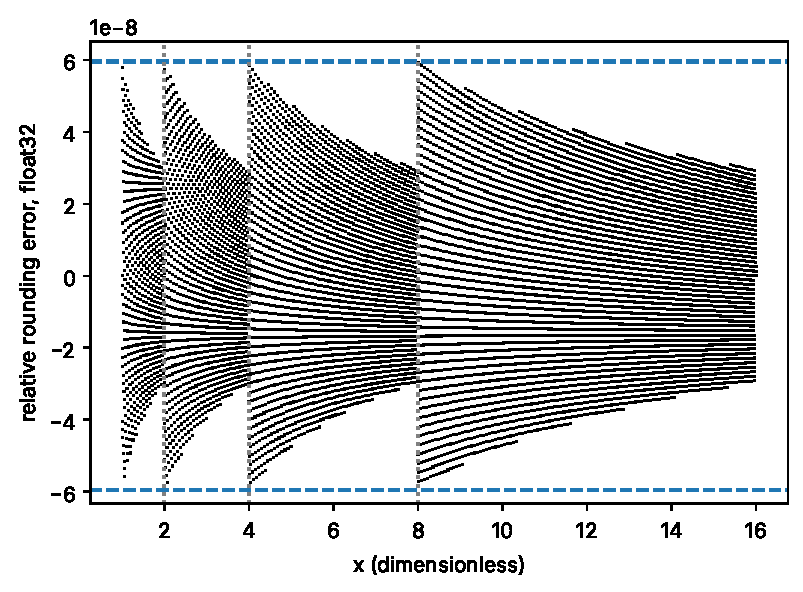
\includegraphics[width=0.85\linewidth]{figs/asymptotics_float.pdf}
\caption{Relative error $(\mathrm{fl}_{32}(x)-x)/x$ of rounding to float32, for $10^4$ values $1\le x\le16$ (dimensionless). The dashed lines are $\pm\varepsilon_{32}/2=\pm5.96\times10^{-8}$. Within each interval $[2^e,2^{e+1})$ the absolute spacing is constant, so the relative error envelope shrinks from $\varepsilon_{32}/2$ to $\varepsilon_{32}/4$ and jumps back at each power of 2 (vertical dotted lines).}
\label{fig:asymptotics-float}
\end{figure}

\subsection{Consequences}

\paragraph{Small additions vanish.} In double precision, $1+10^{-16}$ rounds to exactly 1, since $10^{-16}<\varepsilon/2=1.11\times10^{-16}$. In float32, $1+10^{-8}$ equals 1. And in float32 the integer $16777217=2^{24}+1$ cannot be stored: it rounds to $16777216$.

\paragraph{Accumulation.} Rounding errors add up. Summing $0.1$ ten times gives $0.9999999999999999$ in double and $1.0000001192092896$ in float32. Neither is wrong by more than a few $\varepsilon$, but neither is 1.

\paragraph{Catastrophic cancellation.} Subtracting nearly equal numbers keeps their absolute rounding errors (about $\varepsilon\abs{a}$) but makes the result small, so the \emph{relative} error of the difference is about $\varepsilon\abs{a}/\abs{a-b}$, which can be huge.

\begin{sample}{A harmless rounding error and a catastrophic one}
(a) Compute $\sum_{k=1}^{10}0.1$ in double precision. (b) Compute $(1-\cos x)/x^2$ at $x=10^{-8}$, whose true value is very close to $\tfrac12$.

\textbf{Step 1:} For (a), each addition rounds by \cref{eq:asymptotics-roundmodel}, and $0.1$ itself is stored slightly wrong. The result is $0.9999999999999999$, which differs from 1 by $1.1\times10^{-16}$, half an $\varepsilon$: a harmless error, but enough to make the test \texttt{total == 1.0} fail.

\textbf{Step 2:} For (b), $\cos(10^{-8})=1-5\times10^{-17}+\dots$. The doubles just below 1 are spaced by $\varepsilon/2=1.11\times10^{-16}$, so the nearest double to $1-5\times10^{-17}$ is $1$ itself. The computer gets $\cos x=1$, then $1-\cos x=0$, and the answer $0$.

\textbf{Step 3:} Repair (b) by removing the subtraction analytically: $1-\cos x=2\sin^2(x/2)$, so $(1-\cos x)/x^2=2\sin^2(x/2)/x^2$, which the computer evaluates as $0.5$.

\[
\boxed{\text{(a) }0.9999999999999999,\qquad\text{(b) naive }0,\ \text{rewritten }0.5}
\]
Rule of thumb: never subtract nearly equal floating-point numbers if algebra lets you avoid it, and never test computed numbers with \texttt{==}.
\end{sample}

\subsection{When ``exactly zero'' becomes noise}

Many quantities in physics vanish exactly for a structural reason. For example, certain lists of numbers (eigenvectors, Chapter~\ref{ch:eigen}) have dot product exactly zero, and certain sums cancel term by term in pairs (sum rules, Chapter~\ref{ch:non-hermitian}). On a computer, such a quantity is computed from rounded ingredients and comes out not as 0 but as a small number whose size is set by $\varepsilon$ times the size of the terms that cancel.

A clean example. On a grid of $N$ points, the vectors $\psi_n(j)=\sqrt{2/(N+1)}\,\sin\bigl(nj\pi/(N+1)\bigr)$, $j=1,\dots,N$, are exactly orthonormal: $\sum_j\psi_n(j)\psi_m(j)=0$ for $n\ne m$ (you will prove this in Chapter~\ref{ch:eigen}; they are the eigenvectors of the discrete box). Compute the dot product of $\psi_3$ and $\psi_7$ with $N=999$ by adding the terms in order. In double precision the result is below $10^{-14}$. Store the vectors in float32 and repeat: the result is again small but nonzero, and at least a thousand times larger than the double-precision result; its size is set by $\varepsilon_{32}\approx1.2\times10^{-7}$ times the size of the individual terms. (The exact digits depend on how the platform rounds the sines, so we do not quote them; the listing below prints them.) Nothing is wrong with either computation; the second simply has fewer digits.

The danger comes when such noise is fed to something that can amplify it.

\begin{sample}{A parameter that should do nothing}
A model predicts a correction $p=c\,\eta$ to a quantity, where $c$ is a fitted coefficient and $\eta$ is a sensitivity that is \emph{analytically zero} (the parameter has no physical effect). Because of float32 rounding the computed sensitivity is $\eta=10^{-7}$. A least-squares fit asks for the $c$ that makes $p$ equal a residual $r=0.01$. What does the fit do?

\textbf{Step 1:} Minimizing $(r-c\eta)^2$ over $c$: setting the derivative $-2\eta(r-c\eta)$ to zero gives $c=r/\eta$.

\textbf{Step 2:} With the numbers: $c=0.01/10^{-7}=10^5$.

\textbf{Step 3:} Interpret. The fit ``explains'' the residual perfectly by driving a meaningless parameter to an enormous value. If the noise had come out as $\eta=-3\times10^{-8}$ instead, the same fit would give $c=-3.3\times10^5$. The improvement is real in the computer and meaningless in physics.

\textbf{Step 4:} The repair is to set the analytically zero sensitivity to exactly $0$. Then $p=0$ for every $c$, the fit cannot use the parameter at all, and the coefficient stays where it started (Chapter~\ref{ch:least-squares} explains how such ``null directions'' are handled systematically).

\[
\boxed{c=r/\eta=10^5:\ \text{a huge coefficient harvesting noise}}
\]
\end{sample}

This is, in miniature, what happened in Sec.~V of the paper: the optimizer drove an exactly-null coefficient to $c_0\approx2.2\times10^{6}$ by exploiting float32 noise in analytically zero tensor entries (sensitivity coefficients of the second-order model, Chapter~\ref{ch:non-hermitian}). Chapter~\ref{ch:paper-spurious-floor} dissects the full story.

\begin{pycode}
import numpy as np

total = 0.0
for k in range(10):
    total += 0.1
print(total, total == 1.0)            # 0.9999999999999999 False

x = 1e-8
print((1 - np.cos(x)) / x**2)         # 0.0   (cancellation)
print(2 * np.sin(x / 2)**2 / x**2)    # 0.5   (rewritten)

N = 999
j = np.arange(1, N + 1)
def psi(n, dtype):
    v = np.sqrt(2 / (N + 1)) * np.sin(n * j * np.pi / (N + 1))
    return v.astype(dtype)
for dt in (np.float64, np.float32):
    prod = psi(3, dt) * psi(7, dt)
    # cumsum adds the terms in order, as in the text; np.sum adds
    # pairwise, which hides part of the rounding
    print(dt.__name__, np.cumsum(prod)[-1])   # "zero", in each precision

print(np.finfo(np.float64).eps, np.finfo(np.float32).eps)
\end{pycode}

\begin{pitfall}
Never decide that a computed quantity ``is zero'' by comparing with \texttt{0.0}, and never decide it ``is not zero'' because it prints as $3\times10^{-8}$. Compare it with $\varepsilon$ times the size of the terms that produced it. If theory says a quantity is exactly zero, set it to zero in the code rather than computing it.
\end{pitfall}

\begin{checkpoint}
In float32, is $1+10^{-8}$ different from $1$? In double?
\end{checkpoint}
\checkanswer{In float32 it equals 1, because $10^{-8}<\varepsilon_{32}/2=5.96\times10^{-8}$. In double it is different from 1, because $10^{-8}\gg\varepsilon_{64}/2=1.11\times10^{-16}$.}

\begin{keyideas}
\item Floating-point numbers have about 16 (double) or 7 (float32) significant decimal digits; machine epsilon is $2.2\times10^{-16}$ and $1.2\times10^{-7}$.
\item Each operation rounds with relative error at most $\varepsilon/2$, \cref{eq:asymptotics-roundmodel}; subtraction of nearly equal numbers loses relative accuracy.
\item Analytically zero quantities come out as noise of size $\varepsilon\times$(term size); an optimizer can amplify that noise into large, meaningless parameters.
\end{keyideas}

%======================================================================
\section{Paper connection}\label{sec:asymptotics-paper}
% DYK-BEGIN
\begin{didyouknow}{Newton's Favorite Cubic}
Isaac Newton illustrated his root-finding method around 1669 on the equation $y^3-2y-5=0$, and Joseph Raphson published a streamlined version in 1690. Near a simple root the method roughly doubles the number of correct digits at each step. Much earlier, Heron of Alexandria described an iteration for square roots that is exactly Newton's method applied to $x^2-a=0$.
\end{didyouknow}
% DYK-END

Here is where each tool of this chapter appears in the paper \cite{soniR1}.

\paragraph{Smooth zeros (Sec.~II~A, Eq.~(1), Appendix~A step 2).} The paper defines $s_n$ by $\Nsm(s_n)=n-\tfrac12$ and computes it with ``Brent on $\Nsm(t)=n-\tfrac12$''. \Cref{sec:asymptotics-inverse} showed that this equation has exactly one solution with $s_n>2\pi$ because $\Nsm$ is increasing there, that for $n=1$ it has a second, spurious solution near $0.756$, and that the closed form \cref{eq:asymptotics-sn-lambert} agrees with the root-finder solution. The mean spacing is computed in Appendix~A step 2 as \texttt{np.gradient}(smooth zeros), a finite-difference approximation to the derivative $\dd s_n/\dd n$ of \cref{eq:asymptotics-gap}. For interior indices $20\le n\le999$ the two agree to better than $0.1\%$; at the very first index the one-sided difference $s_2-s_1=6.13$ differs noticeably from the derivative $\gap_1=7.50$. Every rms in the paper is divided by these spacings.

\paragraph{The Lambert-$W$ form (Sec.~I~A, paragraph b).} The paper describes Fran\c ca and LeClair's equation for the $n$-th zero as having a smooth part that ``is the Lambert-$W$ asymptotic of the counting function'' \cite{francaleclair,leclair}. Our \cref{eq:asymptotics-sn-lambert,eq:asymptotics-gap-lambert} are that smooth part, derived in five lines from Eq.~(1).

\paragraph{Precision of the data (Sec.~II~A).} The zeros are computed ``at 20 significant digits'' up to $n=1000$ and ``at 15 digits'' beyond, and the paper says ``both precisions exceed every use below by many orders''. With \cref{sec:asymptotics-errors} you can verify this: the 15-digit value quoted for $t_{1000}$ has rounding error at most $5\times10^{-12}$, about $4\times10^{-12}$ mean spacings (Problem~22), and the paper actually computed zeros up to $1000$ at 20 digits. The smallest errors the paper quotes are of order $10^{-4}$ spacings (the in-sample rms below $10^{-4}$ at $M=900$, Sec.~III), still more than seven orders of magnitude larger.

\paragraph{Inverting the Wu--Sprung potential (Sec.~II~B, Eq.~(2), Appendix~A step 3).} Eq.~(2) gives $x(V)$, an increasing function for $V\ge V_0$ with $V_0=3.10073\pi$. The solver needs $V(x)$; the paper inverts Eq.~(2) ``pointwise by bracketed root finding'' (Sec.~II~B), ``by Brent inversion of Eq.~(2) on a dense reference grid, cubic-spline interpolated'' (Appendix~A step 3). The box half-widths $L=x(1000)=44.883$ and $L=x(1500)=59.957$ are values of the forward function. Chapter~\ref{ch:wu-sprung} derives Eq.~(2).

\paragraph{The oracle's level equation (Sec.~II~D, Appendix~A step 8).} Predicted zeros solve $\Nsm(t)+\Nfl(t)=n-\tfrac12$ by ``Brent bracketed $\pm3$ around the smooth zero (bracket expanded on sign failure)'' (the paper gives no units for the $\pm3$; see \cref{sec:asymptotics-brackets}). This is the bracket-expansion strategy of \cref{sec:asymptotics-brackets}. In Sec.~IV the paper reports that the fitted-amplitude control B with 900 coefficients is ``root-ambiguous (the level equation has several roots for about a third of the held-out levels)'' and that ``the score varies by at most $0.012$ with the choice of root''; this is the non-monotonic situation of \cref{sec:asymptotics-brackets}, flagged with a dagger in Table~IV.

\paragraph{Richardson extrapolation as an asymptotic expansion (Sec.~II~B, Appendix~A steps 3 and 5).} The finite-difference levels behave like $E(h)=E^\ast+ah^2+\order(h^4)$ as the grid spacing $h\to0$ (Chapter~\ref{ch:finite-differences} derives this). Halving $h$ gives $E(h/2)=E^\ast+ah^2/4+\order(h^4)$, and $4E(h/2)-E(h)=3E^\ast+\order(h^4)$, so $(4E(h/2)-E(h))/3$ cancels the $h^2$ term. This is the paper's $E^{\rm Rich}$, built from the ``Richardson pair $12000/24000$'' grids. (The paper writes this combination as $(4E_{2h}-E_h)/3$. The cancellation above works only if the factor $4$ multiplies the levels on the \emph{finer} grid of the pair, so in the paper's formula $E_{2h}$ must be read as the finer-grid levels, our $E(h/2)$. Chapter~\ref{ch:finite-differences} returns to this notation.) Problem~28 practices the idea on a simpler function.

\paragraph{The float32 artifact (Sec.~II~E safeguard (i), Sec.~V, Appendix~A step 9).} The constant mode $\phi_0=1$ of the absorptive-even class has, analytically, zero second-order real shift. Its tensor rows were at first ``left as float32 noise'', and the optimizer ``had driven the exactly-null constant mode to $c_0\approx2.2\times10^{6}$, harvesting in-sample improvement from float32 noise in analytically-zero tensor entries'' (Sec.~V). Before repair the floor was $0.2322$, spuriously close to the PT-odd value $0.2321$; after the rows were ``zeroed analytically'' (Appendix~A step 9) it rose to $0.2358$. The sample ``A parameter that should do nothing'' in \cref{sec:asymptotics-float} is this mechanism in its simplest form; Problem~20 estimates the size of $c_0$ in a quadratic version. Chapter~\ref{ch:paper-spurious-floor} gives the full account.

\paragraph{Asymptotic thinking in the claims.} The paper's statement that the oracle predicts ``essentially as well at $n=10^4$ as at $n=400$'' (Sec.~IV), and its use of heights where the mean spacing is still near 1, both rest on the slow, logarithmic growth of \cref{sec:asymptotics-order,sec:asymptotics-inverse}: between zeros 401 and 10000 the spacing changes only from about 1.3 to about 0.85. (The following is our own remark, not a claim made in the paper: over that range $\log(s_n/2\pi)=2\pi/\gap_n$ grows only from about 4.7 to about 7.4, so ``nearly height-independent'' refers to a modest stretch of the logarithmic scale.)

\begin{keyideas}
\item The paper's smooth zeros, potential inversion and oracle predictions are all bracketed root finding.
\item Lambert $W$ gives the smooth zeros in closed form; the paper cites this form in Sec.~I~A.
\item The spurious result of Sec.~V began as float32 noise in quantities that are exactly zero on paper.
\end{keyideas}

%======================================================================
\section{Summary}\label{sec:asymptotics-summary}

\begin{itemize}
\item Absolute error $\hat x-x$, relative error $(\hat x-x)/x$ (\cref{eq:asymptotics-relerr}); rounding to $d$ significant digits gives relative error $\le5\times10^{-d}$ (\cref{eq:asymptotics-sigdig}). The paper measures errors in mean spacings $\gap_n$.
\item $\order$, $o$, $\sim$ (\cref{eq:asymptotics-bigO,eq:asymptotics-littleo,eq:asymptotics-sim}); $\log t=o(t^a)$ for $a>0$ (\cref{eq:asymptotics-logpower}); $\Nsm(t)\sim\frac{t}{2\pi}\log t$ but converges slowly.
\item Sums of monotone functions lie between integrals (\cref{eq:asymptotics-squeeze,eq:asymptotics-squeeze-inc}); $H_n=\log n+\gamma+\order(1/n)$; $\log n!=n\log n-n+\order(\log n)$ (\cref{eq:asymptotics-lognfact-bounds}).
\item Stirling: $\log n!=n\log n-n+\tfrac12\log(2\pi n)+\vartheta_n/(12n)$, $0<\vartheta_n<1$ (\cref{eq:asymptotics-stirling}); Stirling series \cref{eq:asymptotics-stirling-series}; Gamma function \cref{eq:asymptotics-gamma,eq:asymptotics-gamma-rec}; $\log\Gamma$ asymptotics \cref{eq:asymptotics-stirling-gamma}, extended to complex arguments on trust; preview of $\theta(t)$ \cref{eq:asymptotics-theta}.
\item Inverse functions: existence for strictly monotone continuous functions; $\dd x/\dd y=1/(\dd y/\dd x)$ (\cref{eq:asymptotics-inverse-derivative}); $\Nsm'$, $\Nsm''$ (\cref{eq:asymptotics-nsm-derivs}); $\gap_n=2\pi/\log(s_n/2\pi)$ (\cref{eq:asymptotics-gap}).
\item Lambert $W$ (\cref{eq:asymptotics-lambertw}); $s_n=2\pi(n-\frac{11}8)/W((n-\frac{11}8)/e)$ and $\gap_n=2\pi/(1+W)$ (\cref{eq:asymptotics-sn-lambert,eq:asymptotics-gap-lambert}).
\item Bisection error bound $(b-a)/2^{k+1}$ (\cref{eq:asymptotics-bisect-bound,eq:asymptotics-bisect-steps}); Newton's method and quadratic convergence (\cref{eq:asymptotics-newton,eq:asymptotics-newton-quadratic}); guaranteed monotone convergence for increasing convex $f$; secant method (\cref{eq:asymptotics-secant}); Brent's method as bracketed fast steps.
\item Brackets fail for even root counts, double roots, poles; expand brackets using known monotonicity; non-monotone level equations are root-ambiguous.
\item Floating point (\cref{eq:asymptotics-float}, \cref{tab:asymptotics-formats}): $\varepsilon_{64}=2.2\times10^{-16}$, $\varepsilon_{32}=1.2\times10^{-7}$; rounding model \cref{eq:asymptotics-roundmodel}; cancellation; analytic zeros become noise that fits can amplify.
\end{itemize}

%======================================================================
\section{Problems}\label{sec:asymptotics-problems}

\begin{problemlist}
\prob{1}{The approximation $\pi\approx22/7$ is famous. Find its absolute error, its relative error, and the number of significant digits to which it agrees with $\pi=3.14159265\ldots$.}

\prob{1}{Which of the following are true as $t\to\infty$? (a) $5t^2+3t=\order(t^2)$; (b) $\log t=o(t^{0.1})$; (c) $t\log t\sim t$; (d) $\sin t=\order(1)$; (e) $e^{-t}=o(t^{-100})$.}

\prob{1}{Compute the ratio $\bigl[\frac{t}{2\pi}\log t\bigr]/\Nsm(t)$ at $t=10^6$ and compare with its value $1.64$ at $t_{1000}$ (\cref{sec:asymptotics-order}). What does this say about using the leading-order term?}

\prob{2}{Use \cref{eq:asymptotics-harmonic} to bound $H_{100}$, and compare with the exact value.}

\prob{2}{Use the comparison of sums and integrals for the increasing function $f(x)=x^2$ to show $\frac{n^3}{3}\le\sum_{k=1}^nk^2\le\frac{(n+1)^3-1}{3}$, and deduce $\sum_{k=1}^nk^2\sim n^3/3$.}

\prob{1}{Use Stirling's series \cref{eq:asymptotics-stirling-series} through the $1/(12n)$ term to compute $\log20!$, and find the relative error of the simpler approximation $20!\approx\sqrt{40\pi}\,(20/e)^{20}$.}

\prob{2}{(a) Show from \cref{eq:asymptotics-gamma-rec} that $\Gamma(3)=2$. (b) Using $\Gamma(\tfrac12)=\sqrt\pi$, compute $\Gamma(\tfrac52)$.}

\prob{2}{Apply two steps of Newton's method to $f(x)=x^3-10$ starting from $x_0=2$. Compare with $10^{1/3}$.}

\prob{2}{\emph{(Paper.)} The oracle solver of Appendix~A step 8 starts from a bracket $\pm3$ around the smooth zero; read the $\pm3$ in mean spacings, as \texttt{qmnt} does, so the bracket is $[s_n-3\gap_n,\,s_n+3\gap_n]$. If bisection were used instead of Brent, how many steps would guarantee an error below $10^{-12}$ mean spacings?}

\prob{2}{Show that the integer $2^{24}+1=16777217$ is not representable in float32, and find the float32 value it is stored as. Using numpy, confirm it.}

\prob{2}{Compute $\sqrt{x+1}-\sqrt x$ at $x=10^{12}$ in double precision directly, and again as $1/(\sqrt{x+1}+\sqrt x)$. Find the relative error of the direct method and explain it with \cref{eq:asymptotics-roundmodel}.}

\prob{2}{\emph{(Paper.)} Appendix~A of the paper lists the anchor $t_{500}=811.1843588465$. Find $s_{500}$, $\gap_{500}$ and the fluctuation $(t_{500}-s_{500})/\gap_{500}$.}

\prob{2}{(a) Show that $x\log x=1$ has solution $x=1/W(1)$. (b) Compute $W(1)$ by Newton's method on $g(w)=we^w-1$ from $w_0=0.5$: give $w_1$ and the converged value.}

\prob{2}{\emph{(Computational.)} Using \texttt{qmnt.smooth\_zeros} and \texttt{scipy.special.lambertw}, verify that \cref{eq:asymptotics-sn-lambert} reproduces the smooth zeros for $1\le n\le10^4$. What is the largest discrepancy?}

\prob{3}{Let $a>0$ and $f(x)=x^2-a$. (a) Use the convexity theorem of \cref{sec:asymptotics-newton} to show that Newton's method converges to $\sqrt a$ from every $x_0>0$. (b) Show that $e_{k+1}=e_k^2/(2x_k)$ exactly, where $e_k=x_k-\sqrt a$.}

\prob{2}{\emph{(Computational, paper.)} Using \texttt{qmnt.zeros} and \texttt{qmnt.fluct}, compute the rms of the fluctuations $(t_n-s_n)/\gap_n$ for $401\le n\le500$. Compare with the paper's null $0.263$ on zeros 401--500 (Sec.~II~C, Table~V).}

\prob{2}{For each of the following, say whether $[a,b]$ is a valid bisection bracket and whether bisection would return a root: (a) $f(x)=(x-1)(x-2)$ on $[0,3]$; (b) $f(x)=x^2$ on $[-1,1]$; (c) $f(x)=1/x$ on $[-1,2]$; (d) $f(x)=(x-1)(x-2)(x-3)$ on $[0,4]$.}

\prob{3}{The secant method \cref{eq:asymptotics-secant} has errors that satisfy $e_{k+1}\approx Ce_ke_{k-1}$ near a simple root (you may assume this). Suppose $\abs{e_{k+1}}\approx K\abs{e_k}^q$ for some constants $K,q$. Show that $q$ must satisfy $q^2=q+1$, so $q=(1+\sqrt5)/2\approx1.618$.}

\prob{2}{\emph{(Computational.)} Reproduce the float32 orthogonality experiment of \cref{sec:asymptotics-float} for $N=999$, $n=3$, $m=7$. Then, in the ``parameter that should do nothing'' sample, find $c$ if the computed sensitivity is $\eta=-3\times10^{-8}$ and the residual is $r=0.01$.}

\prob{3}{\emph{(Paper.)} In a second-order model the contribution of a parameter is quadratic, $\delta E=\eta\,c_0^2$, where $\eta$ is an analytically zero tensor entry computed with rounding noise. Suppose (illustratively; these are not the paper's values) $\eta=2\times10^{-14}$ and the optimizer wants $\delta E=0.1$. What $c_0$ does it choose? Compare with the paper's $c_0\approx2.2\times10^{6}$ (Sec.~V) and explain why the fix of Appendix~A step 9 removes the effect.}

\prob{2}{Show that $\gap_n\sim2\pi/\log n$. Compare $\gap_{1000}=1.159$ with $2\pi/\log1000$.}

\prob{1}{\emph{(Paper.)} The paper quotes $t_{1000}=1419.42248094599$. How many significant digits is this? Bound the rounding error of this value in units of $\gap_{1000}=1.159$, and relate your answer to the paper's statement in Sec.~II~A.}

\prob{2}{Apply one Newton step for $s_1$ (i.e. for $f(s)=\Nsm(s)-\tfrac12$) starting from $x_0=7$, just above $2\pi$. Where does it land? Explain, using the convexity theorem, why the iteration still converges.}

\prob{3}{\emph{(Computational, paper.)} Using \texttt{qmnt.oracle\_zeros} with the six primes $2,3,5,7,11,13$ and \texttt{qmnt.score}, compute the held-out rms and correlation on zeros 401--500. Compare with Table~V. Then write your own version with the bracket-expansion listing of \cref{sec:asymptotics-brackets} and \texttt{qmnt.Nfl}, and check that it gives the same predicted zeros.}

\prob{2}{\emph{(Computational.)} Evaluate \texttt{mpmath.siegeltheta(100)} and the three-term approximation $\frac t2\log\frac t{2\pi}-\frac t2-\frac\pi8$ at $t=100$. Show that their difference is close to $1/(48t)$, as \cref{eq:asymptotics-theta} predicts.}

\prob{2}{Let $\gamma_n=H_n-\log n$. Show that $\gamma_n$ is decreasing and positive, and conclude that it converges. (Hint: use $\int_n^{n+1}\dd x/x>1/(n+1)$ and \cref{eq:asymptotics-harmonic}.) Compute $\gamma_{10}$.}

\prob{3}{The equation $v(\log v-1)=n$ (the leading part of $\Nsm(2\pi v)=n$) can be solved by the fixed-point iteration $v_{k+1}=n/(\log v_k-1)$. (a) For $n=1000$ and $v_0=1000$, compute $v_1,\dots,v_4$. (b) Show that near the solution $v^\ast$ the error is multiplied by approximately $-1/(\log v^\ast-1)$ at each step, and evaluate this factor.}

\prob{2}{The symmetric difference quotient $D(h)=(e^h-e^{-h})/(2h)$ approximates $\frac{\dd}{\dd x}e^x\big|_{x=0}=1$ with $D(h)=1+h^2/6+h^4/120+\order(h^6)$. (a) Derive this expansion from the Taylor series of $e^h$. (b) Compute $D(0.1)$, $D(0.05)$ and the Richardson combination $(4D(0.05)-D(0.1))/3$. (c) Predict the error of the combination from the expansion and check it.}

\prob{2}{Keep only the $p=2$, $m=1$ term of the paper's Eq.~(4): $\Nfl(t)=-\frac{1}{\pi\sqrt2}\sin(t\log2)$. Apply one Newton step to $g(t)=\Nsm(t)+\Nfl(t)-\tfrac12$ starting at $t_0=14.5214\approx s_1$, and then find the converged root. Compare with $s_1$ and with $t_1=14.1347$.}

\prob{3}{\emph{(Paper.)} The level equation $\Nsm(t)+\Nfl(t)=n-\tfrac12$ with the six-prime $\Nfl$ of Eq.~(4) ($m\le3$) is certainly monotone where $\abs{\Nfl'(t)}<\Nsm'(t)$. (a) Show that $\abs{\Nfl'(t)}\le\frac1\pi\sum_{p}\sum_{m=1}^3\frac{\log p}{p^{m/2}}$ and evaluate the bound. (b) Compare it with $\Nsm'(800)$. (c) Does your result prove that the oracle's level equation is root-ambiguous? Relate to the root-ambiguous row of Table~IV.}

\prob{2}{\emph{(Computational, paper.)} Using \texttt{qmnt.wu\_sprung\_x} and \texttt{qmnt.wu\_sprung\_V}, compute $x(1000)$ and $x(1500)$, check that \texttt{wu\_sprung\_V} inverts \texttt{wu\_sprung\_x} at these points, and check numerically that $x(V)$ is increasing on $V_0<V\le1500$. Compare with the paper's $L$ values (Sec.~II~B).}
\end{problemlist}

%======================================================================
\section{Answers to selected problems}\label{sec:asymptotics-answers}

\textbf{Problem 1.} $22/7=3.142857$. Absolute error $3.142857-3.141593=1.264\times10^{-3}$. Relative error $1.264\times10^{-3}/3.141593=4.02\times10^{-4}$. The first three digits $3.14$ agree; the fourth ($2$ versus $1$) does not, so $22/7$ agrees with $\pi$ to 3 significant digits. Its relative error $4.0\times10^{-4}$ is just under the 4-digit bound $5\times10^{-4}$ of \cref{eq:asymptotics-sigdig}, but that bound is only a necessary condition: rounded to four digits, $22/7$ gives $3.143$ while $\pi$ gives $3.142$.

\textbf{Problem 2.} (a) True: $5t^2+3t\le8t^2$ for $t\ge1$. (b) True by \cref{eq:asymptotics-logpower} with $a=0.1$. (c) False: $(t\log t)/t=\log t\to\infty$. (d) True: $\abs{\sin t}\le1$. (e) True: $e^{-t}/t^{-100}=t^{100}/e^{t}\to0$ since exponentials beat powers.

\textbf{Problem 3.} At $t=10^6$, $\log(t/2\pi)=13.815511-1.837877=11.977634$, so $\Nsm\approx\frac{t}{2\pi}(11.977634-1)$ (the $\tfrac78$ is negligible here) while $\frac t{2\pi}\log t=\frac t{2\pi}\times13.815511$. The ratio is $1.26$. Even a million units up, the leading term is 26\% too large; it should never be used where accuracy matters.

\textbf{Problem 5.} For increasing $f$, the rectangles of height $f(k)$ on $[k-1,k]$ lie above the curve and those on $[k,k+1]$ lie below it: $\int_{k-1}^{k}x^2\dd x\le k^2\le\int_k^{k+1}x^2\dd x$. Summing over $k=1,\dots,n$: $\int_0^nx^2\dd x=\frac{n^3}{3}\le\sum k^2\le\int_1^{n+1}x^2\dd x=\frac{(n+1)^3-1}{3}$. Dividing by $n^3/3$, both bounds tend to 1, so $\sum k^2\sim n^3/3$. (Exactly, $\sum k^2=n(n+1)(2n+1)/6$.)

\textbf{Problem 6.} $\log20!=20.5\log20-20+\tfrac12\log2\pi+\tfrac1{240}=61.412512-20+0.918939+0.004167=42.335617$, against the exact $42.335616$ (difference $-3.5\times10^{-7}\approx-1/(360\cdot20^3)$). The plain Stirling approximation omits $1/(12n)$ and higher terms, so its ratio to $20!$ is about $e^{-1/240}$; the relative error is about $0.42\%$.

\textbf{Problem 7.} (a) $\Gamma(2)=1\cdot\Gamma(1)=1$, $\Gamma(3)=2\Gamma(2)=2$. (b) $\Gamma(\tfrac32)=\tfrac12\Gamma(\tfrac12)=\tfrac{\sqrt\pi}{2}$ and $\Gamma(\tfrac52)=\tfrac32\Gamma(\tfrac32)=\tfrac{3\sqrt\pi}{4}=1.329340$.

\textbf{Problem 8.} $x_{k+1}=x_k-(x_k^3-10)/(3x_k^2)$. $x_1=2-(8-10)/12=2.166667$. Then $x_1^3=10.171$, so $x_2=2.166667-(10.171296-10)/(3\times2.166667^2)=2.166667-0.171296/14.083333=2.154504$. The exact value is $10^{1/3}=2.154435$, so after two steps the error is $6.9\times10^{-5}$.

\textbf{Problem 9.} The bracket has width $6\gap_n$, and we want $\delta=10^{-12}\gap_n$. By \cref{eq:asymptotics-bisect-steps}, $k\ge\log_2(6\times10^{12})-1=42.45-1=41.45$, so $k=42$ steps are needed. Brent normally needs far fewer than this.

\textbf{Problem 11.} The true value is $1/(\sqrt{x+1}+\sqrt x)=4.99999999999875\times10^{-7}$, and the rewritten form returns exactly this. In the direct form, $\sqrt{10^{12}+1}=10^6+5\times10^{-7}$ must be stored as a double near $10^6$. Doubles near $10^6$ are spaced by $2^{-33}\approx1.16\times10^{-10}$, so by \cref{eq:asymptotics-roundmodel} the stored value can be wrong by up to $5.8\times10^{-11}$. The subtraction of $10^6$ is then exact, so it keeps this absolute error while the result is only $5\times10^{-7}$. The relative error of the direct form is therefore up to about $1.2\times10^{-4}$. Running the code confirms an error of this order, which means roughly 12 of the 16 digits are lost to cancellation.

\textbf{Problem 13.} (a) Put $x=e^u$ as in \cref{eq:asymptotics-xlogx}. Then $ue^u=1$, so $u=W(1)$, and $x=e^{W(1)}=1/W(1)$ (using $W(1)e^{W(1)}=1$). (b) The derivative is $g'(w)=(1+w)e^w$. At $w_0=0.5$: $g=0.5\times1.648721-1=-0.175639$ and $g'=1.5\times1.648721=2.473082$, so $w_1=0.5+0.071020=0.571020$. Further steps converge to $W(1)=0.567143$, which gives $x=1.763223$.

\textbf{Problem 15.} (a) On $(0,\infty)$ we have $f'(x)=2x>0$ and $f''=2>0$, so $f$ is increasing and convex there, with root $\sqrt a$. From any $x_0>0$ the first step gives $x_1=\tfrac12(x_0+a/x_0)>0$, so $x_1$ stays in the interval, and the theorem gives $x_1\ge\sqrt a$. From then on the iterates decrease monotonically to $\sqrt a$. (b) Write the Newton step and subtract $\sqrt a$: $x_{k+1}-\sqrt a=\dfrac{x_k^2+a}{2x_k}-\sqrt a=\dfrac{x_k^2-2\sqrt a\,x_k+a}{2x_k}=\dfrac{(x_k-\sqrt a)^2}{2x_k}$. This is $e_{k+1}=e_k^2/(2x_k)$ exactly.

\textbf{Problem 17.} (a) Not a bracket: $f(0)=f(3)=2>0$, even though the interval contains two roots. (b) Not a bracket: $x^2\ge0$ everywhere, so there is no sign change at the double root. (c) There is a sign change, $f(-1)=-1$ and $f(2)=\tfrac12$, but $f$ is not continuous. Bisection converges to the pole $x=0$, which is not a root. (d) A valid bracket, since $f(0)=-6$ and $f(4)=6$, containing three roots. The first midpoint is $2$, which is itself a root, so bisection returns $2$ immediately.

\textbf{Problem 19.} In double precision the computed dot product is below $10^{-14}$. In float32 it is at least a thousand times larger, at a level set by $\varepsilon_{32}$ times the size of the terms (record the value your machine prints). For the second part, minimizing $(r-c\eta)^2$ gives $c=r/\eta=0.01/(-3\times10^{-8})=-3.33\times10^{5}$. The sign and size of $c$ are set entirely by the noise.

\textbf{Problem 21.} Since $s_n\sim2\pi n/\log n$, we have $\log(s_n/2\pi)=\log n-\log\log n+o(1)$. Dividing by $\log n$ and using $\log\log n=o(\log n)$ (\cref{eq:asymptotics-logpower}) gives $\log(s_n/2\pi)\sim\log n$, so $\gap_n\sim2\pi/\log n$. At $n=1000$, $2\pi/\log1000=0.9096$, while the exact value is $\gap_{1000}=1.159$, a ratio of $1.27$. For comparison, at $n=10^4$ the exact spacing is $\gap_{10^4}=0.854$, against the leading-order value $2\pi/\log10^4=0.682$.

\textbf{Problem 22.} The value has 15 significant digits: four before the decimal point and eleven after it. Rounding error is at most half a unit in the last place, $5\times10^{-12}$, which is $4.3\times10^{-12}$ spacings. The smallest errors the paper quotes are of order $10^{-4}$ spacings (the in-sample rms below $10^{-4}$ at $M=900$, Sec.~III), more than seven orders of magnitude larger, so its statement that the precisions ``exceed every use below by many orders'' (Sec.~II~A) is confirmed. (The paper in fact computed $t_{1000}$ at 20 digits.)

\textbf{Problem 23.} At $x_0=7$: $f(7)=-0.61873$ and $f'(7)=\frac1{2\pi}\log(7/2\pi)=0.017194$. The step is $0.61873/0.017194=35.985$, so $x_1\approx43.0$. The tangent at $x_0$ is nearly flat, so the step is huge. However, it overshoots to the right of $s_1$. By the convexity theorem, every later iterate stays at or above $s_1$ and decreases monotonically to $s_1=14.5213$.

\textbf{Problem 25.} \texttt{mpmath.siegeltheta(100)} returns $87.97216$, and the three-term formula gives $87.97196$. The difference is $2.083\times10^{-4}$, compared with $1/(48\times100)=2.083\times10^{-4}$. They agree to within $10^{-8}$; the next term of \cref{eq:asymptotics-theta} is of order $10^{-9}$.

\textbf{Problem 27.} (a) $v_1=1000/5.907755=169.27$, $v_2=242.04$, $v_3=222.76$, $v_4=226.96$. The iterates oscillate about the solution $v^\ast\approx226.2$. (b) Write $g(v)=n/(\log v-1)$. Then $g'(v)=-n/\bigl(v(\log v-1)^2\bigr)$. At the fixed point, $n/(\log v^\ast-1)=v^\ast$, so $g'(v^\ast)=-1/(\log v^\ast-1)\approx-0.226$. Each step therefore multiplies the error by about $-0.23$, which explains both the oscillation and the steady but linear convergence.

\textbf{Problem 29.} At $t_0=14.5214$: $\Nfl=+0.1346$, $\Nfl'=+0.1251$ and $\Nsm'=0.1333$. Hence $g=0.1346$ and $g'=0.2584$, and one Newton step gives $14.5214-0.5207=14.0007$. Iterating further converges to about $14.021$. Starting from $t_0$, which is $0.387$ above $t_1=14.1347$, the single prime-2 term moves the prediction to within about $0.11$ of $t_1$.

\textbf{Problem 30.} (a) By the chain rule, the derivative of the term $-\frac1\pi\frac{\sin(mt\log p)}{mp^{m/2}}$ is $-\frac1\pi\frac{m\log p\,\cos(mt\log p)}{mp^{m/2}}=-\frac1\pi\frac{\log p\,\cos(mt\log p)}{p^{m/2}}$ (the factor $m$ cancels). The magnitude of a sum is at most the sum of the magnitudes, and $\abs{\cos}\le1$, so $\abs{\Nfl'(t)}\le\frac1\pi\sum_p\sum_{m=1}^3\frac{\log p}{p^{m/2}}$. For $p\in\{2,3,5,7,11,13\}$ the double sum is $6.568$, so the bound is $2.091$. (b) $\Nsm'(800)=\frac1{2\pi}\log\frac{800}{2\pi}=0.771$. (c) The bound exceeds the slope, so this argument does \emph{not} guarantee monotonicity. But the bound assumes all eighteen cosines take their worst values simultaneously, so it does not prove that the equation is root-ambiguous either. The root-ambiguous row of Table~IV is not an oracle row: it is control B with 150 primes and fitted amplitudes. The paper attributes that row's degradation to the underdetermined fit (900 coefficients from 400 zeros). Fitted amplitudes are not bounded by $1/(mp^{m/2})$, so $F'$ can exceed $\Nsm'$. Note that the unfitted 900-term oracle A of Table~IV is not flagged.

\textbf{Problem 31.} \texttt{qmnt.wu\_sprung\_x} gives $x(1000)=44.883$ and $x(1500)=59.957$, the paper's $L$ values for scales 1 and 2 (Sec.~II~B). Feeding these back into \texttt{qmnt.wu\_sprung\_V} returns $1000$ and $1500$ to within $10^{-4}$, so the bracketed root finder undoes the forward map. At the bottom, $x(V_0)=0$, because both $\sqrt{V-V_0}$ and $\log\frac{\sqrt V+\sqrt{V-V_0}}{\sqrt V-\sqrt{V-V_0}}=\log1$ vanish there. On 2000 equally spaced values of $V$ from just above $V_0$ to $1500$, every successive difference of $x(V)$ is positive. This is a numerical check of monotonicity on a grid, not a proof; Chapter~\ref{ch:wu-sprung} discusses the shape of $x(V)$.
